\documentclass[12pt,a4paper]{article}
\usepackage{amsmath,bm} %mathematische Normen
\numberwithin{equation}{section}
\numberwithin{figure}{section}
\usepackage[english]{babel} %neue deutsche Rechtschreibung und Formelsatz
\usepackage{amsfonts} %Zus�tzliche Formeln/Symbole/Sonderzeichen...
\usepackage{amssymb} %Formelsatz
\usepackage{graphicx} %Einbinden von Graphiken
\usepackage{float} %Flussumgebungen
\usepackage[authoryear]{natbib}
%\setcitestyle{authoryear}
\usepackage[font=footnotesize]{caption}
\usepackage{enumerate}
\usepackage[labelfont=bf]{caption}
%\usepackage[utf8]{inputenc} %linux
\usepackage[ansinew]{inputenc} %windows
\usepackage[left=3.0cm,right=2.9cm,top=2.5cm,bottom=2.7cm,includeheadfoot]{geometry}


\date {\today}
\author{Veit L�schow}
\title{Heterogeneous core-mantle boundary heat flux in thermo-chemical core convection}

\begin{document}
\maketitle
\newpage
\tableofcontents
\newpage

\section*{Abstract}

Thermal coupling between convection in Earth's mantle and core was proposed to explain asymmetric features of the geomagnetic field during the history of the Earth. The coupling is caused by laterally varying heat transport from the core to the mantle, induced by lateral temperature gradients in the lower-most mantle. Clues for the temperature gradients were found by seismic tomography.\\
This numerical study aims to explore the influence of these non uniform boundary conditions, as compared to uniform heat flux and isothermal boundary conditions on thermo-chemical core convection and some distinct dynamo properties. \\ 
In our model the heat flux pattern is modeled by a single spherical harmonic of degree and order 2. This setting conserves equatorial symmetry, but imposes azimuthal heat flux gradients. \\
Today, convection in the Earth's core is assumed to be driven predominantly by a combination of thermal and compositional buoyancy sources located at the inner-core boundary. Thermal and compositional diffusivities differ by orders of magnitude. The resulting differences in the dynamical behavior of the two components demand an approach with distinct transport equations and boundary conditions for temperature and chemical concentration. Simulations for five different ratios of thermal and chemical driving are made. \\
We observe that fixed flux conditions promote larger flow scales and an increase of mean kinetic energy densities. The imposed flux pattern locks the outer core flow to the mantle and therefore breaks its azimuthal symmetry, even for relatively low thermal forcing ratios of 20 \%. Despite of the symmetry breaking, stable and dipolar dynamos can be maintained due to the partly chemical forcing with its uniform boundary conditions. Additionally, the chemical component partly adopts to the geometry of the heat flux pattern because advective transport of concentration is more effective in regions of increased heat flux.

\newpage

\section{Introduction and Motivation}

\subsection{A thermo-chemical approach to dynamo modeling}
\subsection{Why use heterogeneous heat flux boundary conditions?}

 
\section{Modeling core convection and dynamo action}

Rotating convection and dynamo action in Earth's core is a topic that has been extensively studied \citep{chandrasekhar1970hydrodynamic}. There exist various ideas of how to formulate a set of equations that depicts all relevant physical processes and that is still as simple and therefore numerically economical as possible. Computation time is the limiting factor when it comes to the question how realistic models of the inner core can be. The gap between the relevant physical parameters expected for the Earth and the parameters that are in range of numerical modeling is still big. It cannot be expected that this gap will be closed only with the help of the increasing computational resources that will become available within the next years. Alternatives to waiting for larger computers that allow to explore earth-like parameters have to be found. Asymptotic models are one possibility already revealing promising results (REFS ???).\\
A question that is closely related to the numerical costs and therefore to the accessible parameter range is the choice of the geometry. Most models are either Cartesian with periodic boundary conditions (BC) or spherical shell models. The latter are of course more realistic for the Earth but numerically more costly and therefore even less earth-like with regard to computational feasible parameters. In this work, a spherical model is used in order to be as earth-like as possible in a geometrical way. As a trade-off, parameter regimes in which Cartesian models could advance, are unreachable here. \\
We model the electrically conducting liquid outer core. It is enclosed by the inner-core boundary (ICB) at the bottom and the core-mantle boundary (CMB) at the top. Convection is driven by destabilizing thermal and compositional gradients across the sphere. For the compositional component, fixed chemical concentrations at the ICB and the CMB are imposed (Derichlet BC). The thermal forcing is maintained by introducing a fixed in - and outflux of heat (Neumann BC). The heat flux at the CMB is laterally heterogeneous, i.e., there exist regions of higher and lower heat flux than lateral average. The inner core and mantle are assumed to be insulating and therefore have no influence on the evolution of magnetic fields. \\ 
In the following all relevant equations are introduced. There exist numerous detailed derivations so that this description will be held relatively short. The according references will be given in each section.\\
\subsection{Frame of reference}
The liquid outer core (LOC) is modeled in a spherical shell with an inner radius R$_i$ and an outer radius R$_o$. It is bounded by the ICB at the bottom the CMB at the top. The shell thickness is chosen according to what is expected for today's state of the Earth and defined over the ratio between R$_i$ and R$_o$: $ a = $ R$_i$ / R$_o$ = 0.35.\\
The LOC is constantly rotating about the z-axis of a Cartesian system. The angular velocity $\Omega$ is invariant in time. The effect of the rotation on the frame of reference will be discussed when it comes to the equation of motion. In the course of this study, spherical coordinates are used. 
\begin{figure}[]
 \begin{minipage}{0.42\textwidth}
  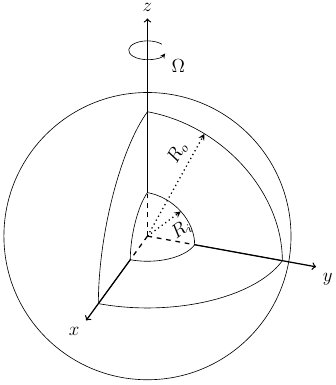
\includegraphics[width=\textwidth]{sketches/spherical_coord.jpg} 
  \caption*{(a)}
 \end{minipage}
 \hfill
\begin{minipage}{0.47\textwidth}
  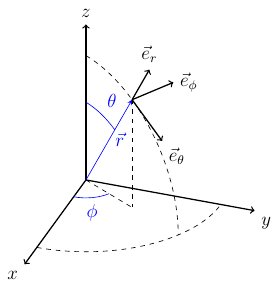
\includegraphics[width=\textwidth]{sketches/spherical_coord2.jpg} 
  \caption*{(b)}
  \end{minipage}
  \caption{(a) Sketch of the liquid outer core. It is bounded by the two spheres of radii R$_i$ and R$_o$. The rotation axis is the cartesian z-axis. (b) This work uses spherical coordinates with unit vectors $ \bm{e_r}$, $\bm{e_\Phi}$ and $\bm{e_\vartheta}$ \citep{trumper2014thermo}.}
\end{figure}
\subsection{Equation of continuity}
\label{sec:continuity}
Per definition, the mass $ \mathcal{M} $ of a material volume $ \mathcal{V}(t) $ with a density $\rho$, moving with a velocity $ \bm u(\bm r,t) $ in a fluid is conserved: 
\begin{equation}
\frac{d \mathcal{M}(\mathcal{V})}{dt} = \frac{d}{dt} \int_{\mathcal{V}(t)} \rho(\bm r,t) d^3r  = 0
\end{equation}
Using Reynold's Transport Theorem and then applying Gauss's Theorem, this yields
\begin{equation}
  \int_{\mathcal{V}(t)} \frac{\partial \rho}{\partial t} d^3r + \oint_{\partial \mathcal{V}(t)} \rho \bm u \cdot \bm {ds} = \int_{\mathcal{V}(t)} \left[ \frac{\partial \rho}{\partial t} + \bm \nabla \cdot (\rho \bm u) \right] d^3r = 0.
\end{equation}
Since this has to hold for all possible material volumes $\mathcal V$, one gets
\begin{equation}
 \frac{\partial \rho}{\partial t} + \bm \nabla \cdot (\rho \bm u) = 0,
\end{equation}
the general form of the equation of continuity. The introduction of the \textit{material derivative} $\frac{D }{Dt} = \frac{\partial }{\partial t} + \bm u \cdot \bm \nabla$ suggests another useful formulation:
\begin{equation}
 \frac{\partial \rho}{\partial t} + \rho \bm \nabla \cdot \bm u + \bm u \cdot \bm \nabla \rho =   \frac{D \rho}{D t} + \rho \bm \nabla \cdot \bm u = 0.
\end{equation}
\subsection{Equation of momentum}
\label{sec:momentum}
In an inertial, non rotating frame of reference, the change of momentum of a material volume $\mathcal{V}$ can be written as 
{\allowdisplaybreaks
\begin{align*}
 \frac{d}{dt} \int_{\mathcal{V}(t)} (\rho u_j) d^3r &= \int_{\mathcal{V}(t)} \left[ \frac{\partial (\rho u_j)}{\partial t} + \frac{\partial}{\partial x_i} (\rho u_j)u_i \right]d^3r \\
    &=   \int_{\mathcal{V}(t)} \left[ \rho \frac{\partial u_j}{\partial t} + u_j \frac{\partial \rho}{\partial t}  +\rho u_j \frac{\partial u_i}{\partial x_i} + u_i \rho \frac{\partial u_j}{\partial x_i} + u_i u_j \frac{\partial \rho}{\partial x_i} \right] d^3r\\
    &= \int_{\mathcal{V}(t)} \left[ u_j\left( \frac{\partial \rho}{\partial t} + \rho \bm \nabla \cdot \bm u + \bm u \cdot \bm \nabla \rho \right) + \rho \left( \frac{\partial u_j}{\partial t} + \bm u \cdot \nabla u_j \right) \right]d^3r \\
    &= \int_{\mathcal{V}(t)}  \rho \frac{D u_j}{D t} d^3r.
\end{align*}}
Change of momentum can happen through either \textit{volume forces} $\bm f$ or \textit{surface forces} $\bm t$:
\begin{equation}
 \int_{\mathcal{V}} \rho \frac{D \bm u}{D t} d^3r = \int_{\mathcal{V}} \bm f d^3r + \oint_{\partial \mathcal{V}} \bm t ds
 \label{eq:force_balance1}
\end{equation}
If a frame of reference is rotating - as in this case - it is no longer an inertial system and therefore pseudo forces have to be expected. Under the assumption of a constant rotation with the angular velocity $\Omega$ and a fixed rotation axis parallel to the Cartesian z-axis, the change of a quantity $\bm P$ in the rotating frame of reference and its change in the non rotating inertial frame relate as
\begin{equation}
\left(\frac{d \bm P}{dt}\right)_F = \left(\frac{d \bm P}{dt}\right)_R + \bm \Omega \times \bm P,
\label{eq:frame_of_reference_rule}
\end{equation}
where the subscripts $F$ and $R$ indicate the \textit{fixed} and the \textit{rotating} frame. Applying rule \eqref{eq:frame_of_reference_rule} twice to a position vector $\bm r$ yields 
\begin{equation}
 \bm a_F = \bm a_R + 2\bm \Omega \times \bm u_R + \bm \Omega \times (\bm \Omega \times \bm r)
 \label{eq:frame_of_reference_accelerations}
\end{equation}
for accelerations $\bm a$. $2\bm \Omega \times \bm u_R$ is the Coriolis force and $\bm \Omega \times (\bm \Omega \times \bm r)$ the centripetal force. \\
With the help of \eqref{eq:frame_of_reference_accelerations}, $\frac{D \bm u}{D t}$ can be transferred from the inertial frame to the frame of reference:
\begin{equation}
 \frac{D \bm u_F}{D t} = \frac{D \bm u_R}{D t} + 2\bm \Omega \times \bm u_R + \bm \Omega \times (\bm \Omega \times \bm r)
 \label{eq:frame_of_reference_material}
\end{equation}
From now on, the subscripts $F$ and $R$ will be cut and all quantities will be measured in the rotating frame. With \eqref{eq:frame_of_reference_material}, \eqref{eq:force_balance1} changes to
\begin{align}
  \int_{\mathcal{V}} \rho \frac{D \bm u}{D t} d^3r = \int_{\mathcal{V}} \bm f d^3r + \oint_{\partial \mathcal{V}} \bm t ds 
  - \int_{\mathcal{V}} \rho \left( 2\bm \Omega \times \bm u + \bm \Omega \times (\bm \Omega \times \bm r) \right) d^3r.
  \label{eq:force_balance2}
\end{align}
Another pseudo force that generally appears in rotating systems, but that is neglected here, is the \textit{Poincar\'{e} force}. Precession driven flows are the most prominent example from geophysics where it plays a dominant role \citep{Tilgner2007}. \\
The \textit{Cauchy Theorem} relates the surface forces $\bm t$ to the stress tensor $\underline{\tau}$ linearly via $\bm t = \underline{\tau} \cdot \bm n$, where $\bm n$ is the normal vector. The surface term in  \eqref{eq:force_balance2} can thus be transformed to
\begin{equation}
 \oint_{\partial \mathcal{V}} \bm t ds = \int_{\mathcal{V}} \bm \nabla \cdot \underline{\tau} d^3r,
\end{equation}
where $\bm \nabla \cdot \underline{\tau} = -\bm \nabla p + \mu \bm \nabla^2 \bm u$ will be used as a reasonable simplification in the context of the Boussinesq approximation (see section \ref{sec:boussinesq}). This expression of $\bm \nabla \cdot \underline{\tau}$ is valid for Newtonian fluids and it is based on the assumption of a solenoidal velocity field ($\bm \nabla \cdot \bm u = 0$) and a homogeneous dynamic viscosity $\mu $ throughout the fluid. \\
The body forces $\bm f$ are the \textit{buoyancy force} $\bm f_g =  \bm g \rho$ and the \textit{Lorentz force} $\bm f_l = \bm j \times \bm B$. The latter will be discussed in section \ref{sec:lorentz}.\\
\par

In the following, the gravitational field $\bm g$ will be discussed in more detail.As mentioned before, the system underlies an asymmetric heat flux at the CMB. This results in an asymmetric temperature field for which the penetration depth of the temperature perturbation to a spherical symmetric solution depends on the amplitude of the heat flux heterogeneity. Following the linear equation of state from the Boussinesq approximation (see section \ref{sec:boussinesq}), this results in a density variation proportional to the temperature variation: $\delta {\rho} \sim \delta {T}$.
\begin{figure}[H]
 \centering
 \includegraphics[scale = 0.24]{sketches/density_var.pdf} 
 \caption{Sketch of the density along the equator, near the CMB. The deviation (black) from the average density (red) results from the asymmetric heat flux at the CMB which has a asymmetric temperature field as an consequence. }
 \label{fig:density_var}
\end{figure}
The total density can be split into one spherical symmetric part $\mathring{\rho}(r)$ that only depends on the radial level $r$ and the density variation due to the heat flux pattern $\delta \mathring{\rho}(r,\vartheta,\phi)$:
\begin{equation}
 \label{eq:density_split}
 \rho(r,\vartheta,\phi) = \mathring{\rho}(r) + \delta \mathring{\rho}(r,\vartheta,\phi).
\end{equation}
In case of a heat flux pattern proportional to the spherical harmonic $\mathcal{Y}_2^2$, the dependence of $\delta \mathring{\rho}$ on $\phi$ is $\pi$-periodic (see Figure \ref{fig:density_var}) so that it can be expressed by the product $\delta \mathring{\rho}(r,\vartheta,\phi) = \mathcal{C}(r,\vartheta) \cdot cos(2\phi)$. $\mathcal{C}$ is only a function of $r$ and $\vartheta$. \\
\textit{Gauss's} gravity law \citep{blakely1996potential} states
\begin{equation}
 \label{eq:gauss}
 \bm \nabla \cdot \bm g = - 4\pi G \rho(r,\vartheta,\phi).
\end{equation}
Integration over a sphere of radius $r$ and application of Gauss's theorem yields
{\allowdisplaybreaks
\begin{align}
% \label{eq:grav_balance}
\nonumber
\int\limits _{\mathcal{V}(r)} \bm \nabla \cdot \bm g dV &= \int\limits_0^\pi \int\limits_0^{2\pi} r^2sin(\vartheta )d\vartheta d\phi \bm g \cdot \bm{e_r}= - 4 \pi G \int\limits_0 ^r \int\limits_0^\pi \int\limits_0^{2\pi} sin(\vartheta) r'^2 \rho(r,\vartheta,\phi) \, dr' d\vartheta d\phi\\
\nonumber
&=- 4 \pi G \int\limits_0 ^r \int\limits_0^\pi \int\limits_0^{2\pi} sin(\vartheta) r'^2 [\mathring{\rho}(r') + \delta \mathring {\rho}(r',\vartheta,\phi)] \, dr' d\vartheta d\phi \\
\nonumber
&=-8\pi^2 G\int\limits_0^r \mathring{\rho}(r') \, dr' -  4 \pi G \int\limits_0 ^r \int\limits_0^\pi sin(\vartheta) r'^2 \mathcal{C}(r',\vartheta) \left( \int\limits_0^{2\pi} cos(2\phi) d\phi \right) \, dr' d\vartheta \\
\nonumber
&= -8\pi^2 G\int\limits_0^r \mathring{\rho}(r') \, dr'
\end{align}}
Because the integration of $\delta \mathring {\rho}(r',\vartheta,\phi)$ over $\phi$ drops out for every value of $r$ and $\vartheta$, $\bm g$ can be expressed by
\begin{equation}
\label{eq:gravity_field}
 g(\bm r) = -\frac{4 \pi G}{r^2}\int_0^r \mathring{\rho}(r')r'^2 \, dr
\end{equation}
and it is worth noticing that $\bm g$ has the same form as in the spherical symmetric case \citep{blakely1996potential}.\\
The buoyancy force term $\bm g \rho$ will be further discussed in section \ref{sec:boussinesq}.

\subsection{Maxwell equations, Lorentz force and induction equation}
\label{sec:lorentz}
The liquid outer core consists of a metallic and therefore conducting fluid. Electric currents may evolve, create magnetic fields and these again may generate currents and influence the flow field. The induction equation is a transport equation for a magnetic fields $\bm B$ 'hosted' by a fluid moving with a velocity $\bm u$. The Lorentz force characterizes the influence of the magnetic field on the flow field, whereas the Maxwell equations describe how electric and magnetic fields interact through charges and currents. They form a basis for the 'magnetic part' of Magnetohydrodynamics (MHD).\\
In the scope of core convection, a reduced form of the Maxwell equations (Pre-Maxwell equations) suffices \citep{davidson2001introduction}: 
\begin{subequations} \label{eq:maxwell}
\begin{align}
 \label{eq:ampere}
 \bm \nabla \times \bm B &= \mu_0 \bm j \quad & \text{(Amp\`{e}re's law)} \\
 \label{eq:charge_conservation}
 \bm \nabla \cdot \bm j &= 0 \quad & \text{(Charge conservation)}\\
\label{eq:faraday}
 \bm \nabla \times \bm E &= - \frac{\partial \bm B}{\partial t} \quad & \text{(Faraday's law)}\\
 \label{eq:no_magnetic_monopoles}
 \bm \nabla \cdot \bm B &= 0 \quad & \text{(No magnetic monopoles)} 
\end{align}
\end{subequations}
Additionally, an extended version of \textit{Ohm's law} for moving conductors
\begin{equation}
\label{eq:ohm}
 \bm j = \sigma (\bm E + \bm u  \times \bm B)
\end{equation}
and an expression for the \textit{Lorentz force}
\begin{equation}
\label{eq:lorentz}
 \bm f_l = \bm j \times \bm B = \frac{1}{\mu_0} (\bm \nabla \times \bm B \times \bm B)
\end{equation}
are needed. $\bm E$ describes the electric field, $\bm j$ the current density, $\mu_0$ the vacuum permeability and $\sigma$ the conductivity of the fluid.\\
The \textit{induction equation}, a transport equation for the magnetic field, can be derived using \eqref{eq:faraday}, \eqref{eq:ohm} and the solenoidal character of $\bm B$ \eqref{eq:no_magnetic_monopoles} and $\bm u$:
\begin{equation}
 \label{eq:induction}
 \frac{\partial \bm B}{\partial t} = \bm \nabla (\bm u \times \bm B) + \eta \bm \nabla^2 \bm B,
\end{equation}
where $\eta = \frac{1}{\sigma \mu_0}$ is the magnetic diffusivity.

\subsection{Conservation of energy and the light component}
\label{sec:internal_energy}
The conservation of internal energy in a fluid reads
\begin{equation}
 \label{eq:internal_energy}
 \rho \frac{D e}{D t} =  -\bm \nabla \cdot \bm q_\textrm{\tiny T} - p(\bm \nabla \cdot \bm u) + \Phi,
\end{equation}
where the internal energy per unit mass is described by $e$. It can be changed by either \textit{volume compression} $- p(\bm \nabla \cdot \bm u)$, \textit{viscous dissipation} $\Phi$ or a \textit{heat flux} $\bm q_\textrm{\tiny T}$ through the fluid surface. In the context of the Boussinesq approximation (section \ref{sec:boussinesq}), viscous dissipation $\Phi$ is negligible and $\bm \nabla \cdot \bm u = 0$. Furthermore, using the \textit{Fourier law} $ \bm q_\textrm{\tiny T} = - k_\textrm{\tiny T} \bm \nabla T$ and the \textit{perfect gas} approximation $e = c_\textrm{\tiny P} T$, \eqref{eq:internal_energy} can be transformed to 
\begin{equation}
 \label{eq:heat_equation}
 \frac{D T}{D t} = \kappa_\textrm{\tiny T} \bm \nabla^2 T.
\end{equation}
Here, $\kappa_\textrm{\tiny T} = \frac{k}{c_\textrm{\tiny P} \rho}$ is the thermal diffusivity and $T$ the fluid temperature. Internal sources of $e$ in the liquid outer core are completely omitted in this study.\\
The derivation of equation \eqref{eq:heat_equation} was adopted from \citet{kundu2008fluid}.\\
\\
The light component is released at the ICB as the inner core slowly crystallizes. It serves as an additional source of buoyancy. In this model, the light component per unit mass, $C$, can only change by a flux $\bm q_\textrm{\tiny C}$ through the surface of the fluid. According to the equation for the conservation of the internal energy above,
\begin{equation*}
 \rho \frac{D C}{Dt} = - \bm \nabla \cdot \bm q_\textrm{\tiny C}
\end{equation*}
can be transformed to 
\begin{equation}
\label{eq:chemical_equation}
 \frac{D C}{D t} = \kappa_\textrm{\tiny C} \bm \nabla^2 C,
\end{equation}
using $\bm q_\textrm{\tiny C} = - k_\textrm{\tiny C} \bm \nabla C$ and introducing $\kappa_\textrm{\tiny C} = \frac{k_\textrm{\tiny C}}{\rho}$.
\subsection{The Boussinesq approximation}
\label{sec:boussinesq}
In most geophysical applications of fluid dynamics, the Boussinesq approximation is a reasonable simplification of the full equations. \\
Starting from an adiabatic reference state, density, pressure, temperature and composition can be separated into a reference state value (denoted by an overbar) that is only dependent on the radial level $r$ and a fluctuating part (denoted by a prime):
\begin{align}
 T = \bar T(r) + T', \quad C = \bar C(r) + C', \quad 
 \rho = \bar \rho(r) + \rho', \quad p = \bar p(r) + p' 
\end{align}
Further on, it is assumed that the typical length scale of the system (here: the shell thickness $d$) is small compared to the scale heights in the reference state. Perturbations to that state shall be small compared to the adiabat. As a result, the reference state becomes independent of position.\\ 
Whether the assumption of a negligible small superadiabaticity is valid in the context of core convection is still debated \citep{anufriev2005boussinesq}. The alternative is to model either the fully compressible equations or to use the anelastic approximation that, in contrast to the Boussinesq model, allows density stratification. \citet{jones2007thermal} extensively discusses the implications of the choice of one of these approaches.\\
From the Boussinesq approximation it follows for the system of equations that
\begin{itemize}
 \item[-] the equation of state takes a linear form: 
 \begin{equation}
  \rho' = -\bar \rho (\alpha_\textrm{\tiny T} T' + \alpha_\textrm{\tiny C} C'), 
 \end{equation}
 where $\alpha_\textrm{\tiny T}$, and $\alpha_\textrm{\tiny C}$ signify the thermal and compositional expansion coefficient.
 \item[-] the equation of continuity transforms to
\begin{equation}
\label{eq:incompressible}
 \bm \nabla \cdot \bm u = 0 \quad \quad \quad \quad \text{(solenoidal character of } \bm u ).
\end{equation}
\item[-] the dissipative heating term can be neglected in the equation of momentum and internal energy (see section \ref{sec:momentum} and \ref{sec:internal_energy}).
\item[-] the material properties such as $\alpha_\textrm{\tiny T}$, $\alpha_\textrm{\tiny C}$, $\mu_0$, $c_\textrm{\tiny P}$, $\eta$, $\kappa_\textrm{\tiny T}$ and $\kappa_\textrm{\tiny C}$ stay constant throughout the fluid.
\end{itemize}
An important advantage of the modified equations is that sound waves are \textit{filtered out}. This reduces the numerical costs without curtailing any relevant physical processes, since the short time scales of sound waves does not have to be resolved numerically.\\
In the differential form, the equation of momentum \eqref{eq:force_balance2} now reads
\begin{equation}
 \frac{D \bm u}{D t} = -2\bm \Omega \times \bm u  - \bm \nabla \left( \frac{\pi'}{\bar \rho} \right) + \nu \bm \nabla^2 \bm u + \frac{1}{\mu_0 \bar \rho}(\bm \nabla \times \bm B) \times \bm B + \frac{\bm g}{\bar \rho} \rho',
\label{eq:force_balance3}
\end{equation}
where $\nu = \mu/\bar \rho$ is the new kinematic viscosity. The centrifugal potential is incorporated into the pressure fluctuation term $\pi' = p' - \frac{\bar \rho \Omega^2 s^2}{2}$, where $s$ is the distance from the z-axis in cylindrical coordinates. The hydrostatic pressure gradient of the reference state $\bm \nabla \bar p$ is balanced by the gravity force $\bm g \bar \rho$ so that only $\rho'$ appears equation \eqref{eq:force_balance3}.\\
\subsection{Boundary conditions}
\label{sec:bc}
This section is dedicated to the boundary conditions.\\ 
For the velocity field they are chosen to be \textit{no-slip}, e.g. $\bm u = 0$ on the ICB ($r = R_i$) and the CMB ($r =R_0$), in order to be comparable to other studies. Several authors state that these \textit{rigid} BC reflect what is realistic for the interaction between the inner and outer core and the outer core and the mantle, respectively \citep{glatzmaier1995three, christensen2006scaling, trumper2012numerical}. On the other hand, \citet{zhang1987onset} or \citet{kuang1997earth} argue that the Ekman layers which result from rigid boundaries are be negligibly thin in the Earth's core due to its extremely small viscosity. Because today's numerical models are forced to use a far to high viscosity, they over emphasize the effect of Ekman layers and therefore \textit{stress-free} BC are more appropriate. For a better comparison, this work follows the approach that was used by related studies \citep{olson2002time, aubert2008thermochemical, hori2014ancient}. \\
According to \citet{trumper2012numerical}, Derichlet type BC are chosen for the chemical component. A compositional gradient, $\Delta C = C'_\textrm{\tiny ICB} - C'_\textrm{\tiny CMB}$, is imposed across the shell. In a more earth-like scenario, one would apply Neumann type conditions with fixed compositional influx at the ICB and zero outflux at the CMB \citep{braginsky1995equations}. This would further increase the complexity of the model and is therefore adjourned in this case. \\
The mantle is assumed to be an insulator due to its rocky content \citep{dormy1998mhd}. The question whether the inner core should be treated as an insulator or not was discussed by \citet{wicht2002inner}. He found that the effect of a conducting inner core on the flow field and the magnetic field is rather small. It is hence reasonable to choose $\sigma = 0$ in the inner core in order not to be obliged to solve the induction equation in the full sphere. In the mantle and the core, the magnetic field $\bm B$ is the solution to 
\begin{equation}
 \label{eq:mag1}
 \bm B = - \bm \nabla \Phi
\end{equation}
with $\Phi$ being a scalar potential that follows the Laplace equation 
\begin{equation}
 \label{eq:mag2}
 \bm \nabla ^2 \Phi = 0.
\end{equation}
The BC are expressed through the fact that $\bm B$ has to match the solution of \eqref{eq:mag1} at the ICB and the CMB.\\
The thermal BC is of the Neumann type and will be discussed in more detail in the following section.
\subsection{CMB - heat flux pattern}
\label{sec:flux_pattern}
A heat flux balance between the inner and the outer core boundary is assumed. The total influx at the ICB Q$_i$ equals the total outflux Q$_o$ at the CMB:
\begin{align}
 -\textrm{Q}_i &= \textrm{Q}_o\\
 \Leftrightarrow \int \limits_{\mathcal{S}_\textrm{\tiny{ICB}}} \kappa_\textrm{T} \nabla T\big|_\textrm{\tiny{ICB}} \cdot \bm{e_r} \, dS &= \int \limits_{\mathcal{S}_\textrm{\tiny{CMB}}} \kappa_\textrm{T} \nabla T\big|_\textrm{\tiny{CMB}} \cdot \bm{e_r} \, dS \\
 \label{eq:fluxbalance1}
 \Leftrightarrow \int \limits_{\mathcal{S}_\textrm{\tiny{ICB}}} \frac{\partial T}{\partial r} \bigg|_\textrm{\tiny{ICB}} \, dS &= \int \limits_{\mathcal{S}_\textrm{\tiny{CMB}}} \frac{\partial T}{\partial r} \bigg|_\textrm{\tiny{CMB}} \, dS 
\end{align}
For the spectral decomposition it is important to notice that only the 0th order spherical harmonic $\mathcal{Y}_0^0$ yields values $\neq$ 0 when being integrated over a closed surface $\mathcal{S}$:
\begin{align}
\nonumber
 \int \limits_{\mathcal{S}} \frac{\partial T}{\partial r} \, dS = \int \limits_{\mathcal{S}} \left(\frac{\partial T}{\partial r}\right)_0^0 \mathcal{Y}_0^0 \, dS,
\end{align}
with $\left(\frac{\partial T}{\partial r}\right)_0^0$ being the spectral coefficient of degree and order 0.
Thus, \eqref{eq:fluxbalance1} can be transformed into the spectral domain via
\begin{align}
\nonumber
 \int \limits_{\mathcal{S}_\textrm{\tiny{ICB}}} \left(\frac{\partial T}{\partial r}\right)_0^0\bigg|_\textrm{\tiny{ICB}} \mathcal{Y}_0^0 \, dS &=  \int \limits_{\mathcal{S}_\textrm{\tiny{CMB}}} \left(\frac{\partial T}{\partial r}\right)_0^0\bigg|_\textrm{\tiny{CMB}} \mathcal{Y}_0^0 \, dS\\ 
 \nonumber
 \Leftrightarrow \left(\frac{\partial T}{\partial r}\right)_0^0\bigg|_\textrm{\tiny{ICB}}  R_i^2 &= \left(\frac{\partial T}{\partial r}\right)_0^0\bigg|_\textrm{\tiny{CMB}} R_o^2.
\end{align}
This allows to formulate a simple relation between the mean radial temperature gradient at the inner and outer boundary:
\begin{equation}
\label{eq:beta_relation}
\left(\frac{\partial T}{\partial r}\right)_0^0\bigg|_\textrm{\tiny{ICB}} = \left(\frac{\partial T}{\partial r}\right)_0^0\bigg|_\textrm{\tiny{CMB}} \frac{R_o^2}{R_i^2} = - \beta \frac{R_o^2}{R_i^2} = - \beta \frac{1}{a^2}
\end{equation}
with $\beta := - \left(\frac{\partial T}{\partial r}\right)_0^0\bigg|_{\textrm{\tiny{CMB}}}$ as prescribed temperature gradient of degree and order 0 at the CMB.\\
Since no internal sources of heat are assumed, the stationary form of \eqref{eq:heat_equation} takes the form of a Laplace equation. It reads
\begin{equation}
 \nabla ^2 T = 0 \label{eq:laplace}
\end{equation}
and with \eqref{eq:beta_relation} the appropriate BC are
\begin{equation}
 \textrm{at the ICB:} \quad  \frac{\partial T}{\partial r}\bigg|_{\textrm{\tiny{ICB}}} = - \beta \frac{1}{a^2} \mathcal{Y}_0^0 \label{eq:BCicb}
\end{equation}
\begin{equation}
  \textrm{at the CMB:} \quad \frac{\partial T}{\partial r}\bigg|_{\textrm{\tiny{CMB}}} = - \beta \mathcal{Y}_0^0 + Amp_l^m \mathcal{Y}_l^m \label{eq:BCcmb}.
\end{equation}
$Amp_l^m$ is the amplitude of the heat flux heterogeneity for a heat flux pattern $\mathcal{Y}_l^m$. Its definition follows the work of \citet{hori2014ancient}:
\begin{equation}
 Amp = \frac{q_\textrm{\tiny{max}} - q_\textrm{\tiny{min}}}{2q_\textrm{\tiny{mean}}}
\end{equation}
The mean heat flux at the CMB $q_\textrm{\tiny{mean}}$ results from the temperature gradient $\beta$ at the CMB. $q_\textrm{\tiny{max}}$ and $q_\textrm{\tiny{max}}$ are the extrema of the lateral heat flux variation.  \\
\\
In order to implement the BC into the numerical model, a (conductive) solution to \eqref{eq:laplace} has to be found. In the most general form, it reads
\begin{equation}
 T = \sum \limits_{l,m} \left[ a_l^m r^l + b_l^m r^{-l-1} \right] \mathcal{Y}_l^m(\vartheta,\phi) \label{eq:cond}
\end{equation}
and its radial derivative 
\begin{equation}
\frac{\partial T}{\partial r} = \sum \limits_{l,m} \left[l a_l^m r^{l-1} - (l+1) b_l^m r^{-l-2}\right]  \mathcal{Y}_l^m(\vartheta,\phi). \label{eq:gradcond}
\end{equation}
At the ICB, \eqref{eq:BCicb} and \eqref{eq:gradcond} yield
\begin{equation}
 - b_0^0 R_i^{-2} = -\beta \frac{1}{a^2} \quad \Rightarrow \quad b_0^0 = \beta R_o^2
\end{equation}
for $l=m=0$ and the algebraic equation 
\begin{equation}
 la_l^m R_i^{l-1} - (l+1) b_l^m R_i^{-l-2} = 0 \label{eq:algebraicICB}
\end{equation}
follows for all $l>0$ and $m>0$.\\
For the  CMB, \eqref{eq:BCcmb} and \eqref{eq:gradcond} yield
\begin{equation}
 l a_l^m R_o^{l-1} - (l+1)b_l^m R_o^{-l-2} = Amp_l^m. \label{eq:algebraicCMB}
\end{equation}
Since only a heat flux pattern with $l=m=2$ will be used here, \eqref{eq:algebraicICB} and \eqref{eq:algebraicCMB} simplify to a linear system of equations
\begin{equation}
 \left( \begin{matrix} 2R_o & -3R_o^{-4}\\ 2R_i & -3R_i^{-4}\end{matrix} \right) \left(\begin{matrix} a_2^2\\b_2^2 \end{matrix}\right) = \left( \begin{matrix} Amp_2^2 \\ 0 \end{matrix} \right).                                                                                                                                                
\end{equation}
Inserting $a_2^2$, $b_2^2$ and $b_0^0$ into \eqref{eq:cond} gives a solution to \eqref{eq:laplace} that respects the boundary conditions \eqref{eq:BCicb} and \eqref{eq:BCcmb}:
\begin{equation}
 T_\textrm{cond}(r,\vartheta,\phi) = \left( a_0^0 + \frac{R_o^2 \beta}{r} \right) \mathcal{Y}_0^0 + Amp_2^2\cdot \frac{R_o^22a^5r^3 - 3R_o^2(a-1)^5r^2}{6D^4(a-1)^2(1-a^5)} \mathcal{Y}_2^2(\vartheta,\phi)
\end{equation}
$a_0^0$ is an arbitrary integration constant that is chosen to be 0 in the following. This conductive temperature profile with its spherically asymmetric part will be introduced into the equations in the density fluctuation part $\rho'$ in section \ref{sec:cond_conv}. \\
\par
The effect of the CMB - heat flux pattern on the conductive temperature field is shown in Figure \ref{fig:conductives}(a) and (b). Regions, where the heat flux from the core to the mantle is increased (heat flux maxima are located at 90$^\circ$ and 270$^\circ$ east, see also the sketch in Figure \ref{fig:fluxsketch}), are characterized by relatively low temperatures because they are cooled more effectively. Vice versa, regions of reduced heat flux (heat flux minima are located at 0$^\circ$ and 180$^\circ$) show higher temperatures than average. 
\begin{figure}[t]
 \begin{minipage}{0.36\textwidth}
  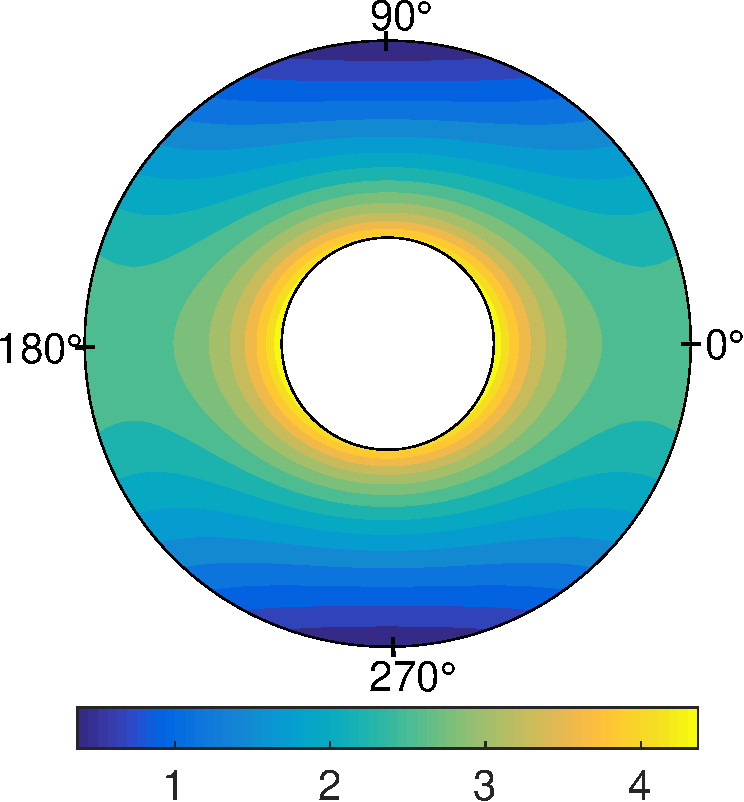
\includegraphics[width=0.9\textwidth]{graphs/theory/temp_field1-crop.pdf}
  \caption*{(a) Equatorial view}
 \end{minipage}
 \hfill
 \begin{minipage}{0.62\textwidth}
  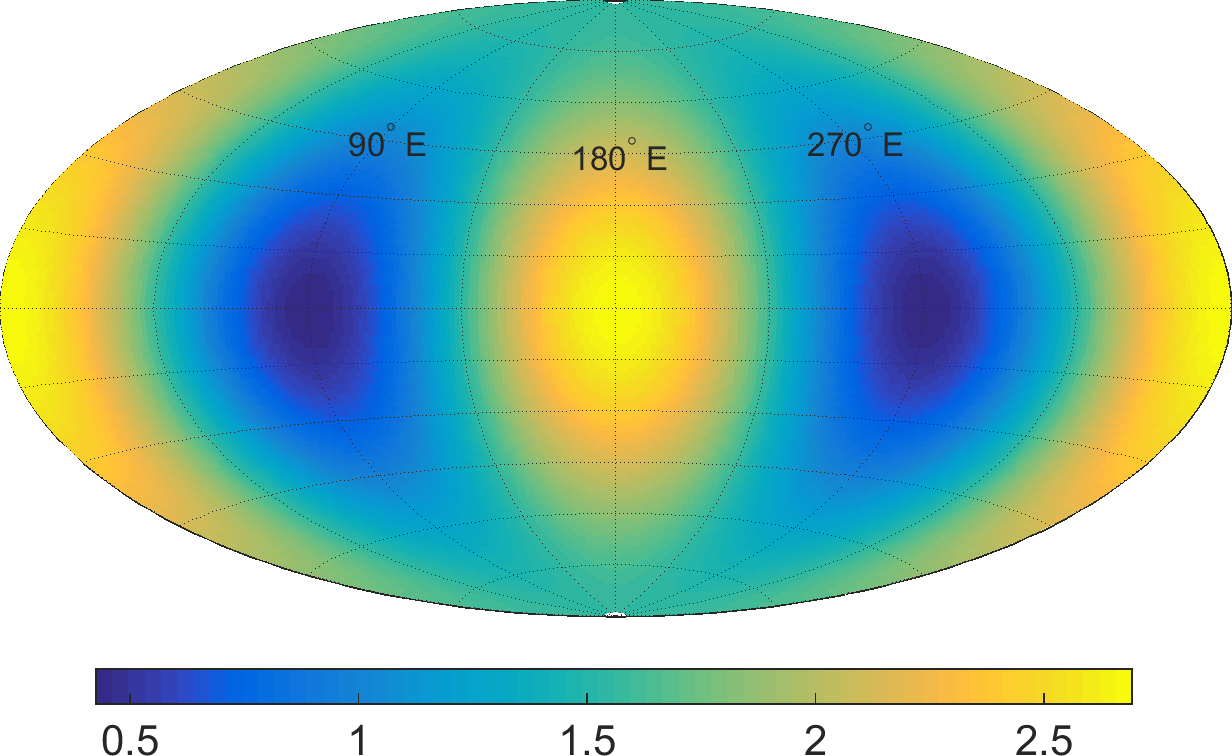
\includegraphics[width=0.9\textwidth]{graphs/theory/temp_field2-crop.png}
  \caption*{(b) Surface projection}
 \end{minipage}
\caption{Conductive temperature field $T_\textrm{cond}$ in the equatorial plain (left) and as a \textit{Hammer-Aitov-projection} at the CMB (right) in a non dimensional form (see section \ref{sec:nondim}). The amplitude of the heat flux heterogeneity is $Amp_2^2 = 1$, heat flux maxima are located at 90$^\circ$ and 270$^\circ$, respectively. See Figure \ref{fig:fluxsketch} for a schematic overview. } 
\label{fig:conductives}
\end{figure}
\\
\\
The amplitude of heterogeneity, $Amp_2^2$, from now on referred to as $q^*$, plays a central role for the heat flux pattern. Figure \ref{fig:equator_flux} shows the core-mantle heat flux along the equator for two values of $q^*$. If the amplitude is chosen to be greater than 1, negative (inward) heat flux occurs in distinct regions around the flux minima. Heat flow from the mantle to the core produces gravitationally stable regions with respect to temperature. Together with an always destabilizing compositional gradient, this could yield non linear double-diffusive effects as fingering or layering. A scenario in which gravitationally stable regions play a role in core convection was recently discussed for mercury \citep{tian2015magnetic}. Yet for the Earth, where the heterogeneities in core-mantle heat flux are considered to be rather mild \citep{aubert2008thermochemical, olson2002time, glatzmaier1999role}, \citet{nakagawa2008lateral} expect that heat flows from the mantle to the core where compositionally dense piles settle at the base of the mantle. Because of that and due to the fact that this study aims to explore the effect of a heat flux pattern on core convection from a general perspective, values of $q^* >1$ are likewise regarded.
\begin{figure}[H]
 \begin{minipage}[left]{0.7\textwidth}
  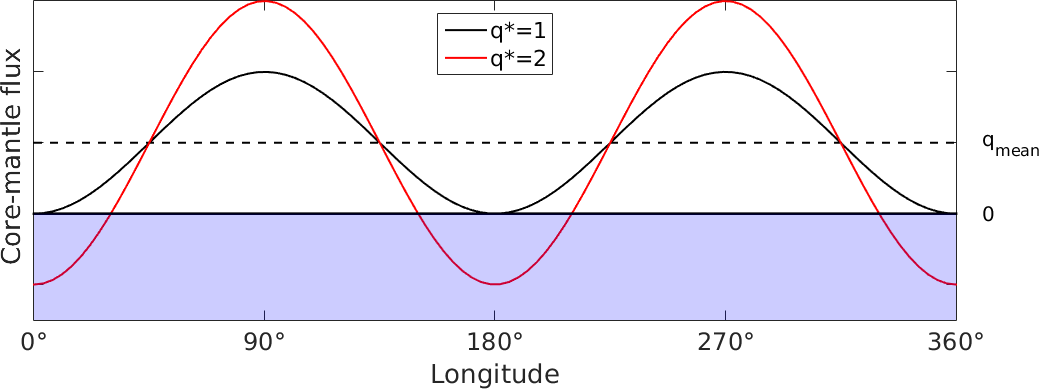
\includegraphics[width=1\textwidth]{sketches/eq_flux-trim.png}
\caption{Plot of the CMB - heat flux along the equator for amplitudes of heterogeneity $q^* = 1$ and $q^* = 2$. For $q^* > 1$, heat partially flows from the mantle to the core (blue region). } 
 \label{fig:equator_flux}
 \end{minipage}
 \hfill
  \begin{minipage}[right]{0.25\textwidth}
  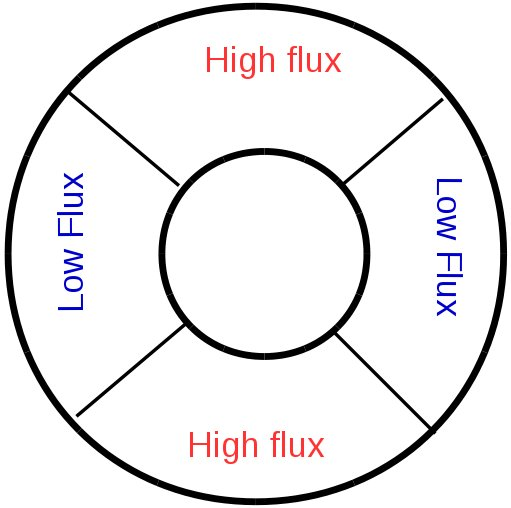
\includegraphics[width=0.92\textwidth]{sketches/pattern.jpg}
 \caption{Sketch of the equatorial plain and the distribution of high and low heat flux at the CMB. }
 \label{fig:fluxsketch}
  \end{minipage}
\end{figure}
\subsection{Non dimensional equations}
\label{sec:nondim}
A common procedure in fluid dynamics is to \textit{rescale} the equations introduced so far in order to reduce the number of parameters and to make the relevant physical processes intuitively more accessible. The new scales are adopted from \citet{trumper2012numerical}, they are summarized in table \ref{tab:scales}.
\begin{table}[H]
\centering
\begin{tabular}{ccc}
 Variable & Symbol & Scale\\
 \hline
 Length	& $\bm r$ & $D =R_o - R_i$\\
 Time	&$t$	  & $D^2/\nu$\\
 Velocity & $\bm u$ & $\nu / D$\\
 Temperature & $T$ & $ \beta D$\\
 Composition & $C$ & $\Delta C$ \\
 Pressure & $\pi$ & $\bar \rho \nu^2/D^2$\\
 Magnetic Field & $\bm B$ & $\sqrt{\eta \Omega \mu_0 \bar \rho}$\\
 \end{tabular}
 \caption{Overview of the the new scales that are introduced to non dimensionalize the magnetohydrodynamic system of equations that was introduced in the sections \ref{sec:continuity} to \ref{sec:boussinesq}.}
 \label{tab:scales} 
\end{table}
The application of these scales to \eqref{eq:incompressible}, \eqref{eq:force_balance3}, \eqref{eq:heat_equation}, \eqref{eq:chemical_equation} and \eqref{eq:induction} yields a system of non dimensional equations:
{\allowdisplaybreaks
\begin{subequations} \label{eq:nondim}
 \begin{align}
\label{eq:incompressible^}
{\bm {\hat \nabla}} \cdot \bm{ \hat u} = & \quad0, \\
\label{eq:momentum^} \nonumber
\frac{D \bm{ \hat u}}{D \hat t} = &- \bm{ \hat \nabla} \hat \pi' - \frac{2}{\textrm{Ek}}\, \bm{e_z} \times \bm{ \hat u} + \bm{ \hat \nabla}^2 \bm{ \hat u} + \frac{1}{\textrm{Ek}  \textrm{Pr}_\textrm{\tiny{m}}} \left( \bm{ \hat \nabla} \times \hat{ \bm B} \right) \times \hat{ \bm B}  \\ 
 &+ (\textrm{Ra}_\textrm{\tiny {T}} \hat{ T'} + \textrm{Ra}_\textrm{\tiny {C}} \hat{ C'} )(1-a) \hat{r} \, \bm{e_r}, \\
\label{eq:heat_equation^}
 \frac{D \hat T'}{D t} =& \quad \frac{1}{\textrm{Pr}_\textrm{\tiny T}} \bm{\hat \nabla}^2 \hat T',\\
 \label{eq:chemical_equation^}
 \frac{D \hat C'}{D t} =& \quad \frac{1}{\textrm{Pr}_\textrm{\tiny C}} \bm{\hat \nabla}^2 \hat C' \textrm{ and}\\
  \label{eq:induction^}
 \frac{\partial \bm {\hat{B}}}{\partial \hat t} = & \quad  \bm{\hat \nabla} \times (\bm{\hat u} \times \bm{\hat{B}}) + \frac{1}{\textrm{Pr}_\textrm{\tiny m}} \hat{ \bm \nabla}^2 \bm{\hat {B}}.
 \end{align}
\end{subequations}}\\
Nondimensional quantities are denoted by \^{} and they are related to their dimensional counterparts via $(\textrm{ }) = \textit{scale } \hat{(\textrm{ })}$. \\
The following parameters of similarity appear in the equations:
{\allowdisplaybreaks
 \begin{align}
\nonumber 
&\textrm{Thermal Rayleigh number : } &\textrm{Ra}_\textrm{\tiny {T}} = \frac{\alpha_\textrm{\tiny T} g \beta D^4}{\nu^2} \\ \nonumber 
%  \\ \nonumber 
&\textrm{Compositional Rayleigh number : } &\textrm{Ra}_\textrm{\tiny C} = \frac{\alpha_\textrm{\tiny C} g \Delta C D^3}{\nu^2} \\ \nonumber 
%  \\ \nonumber 
 &\textrm{Ekman number : }   & \textrm{Ek} = \frac{\nu}{\Omega D^2} \\ \nonumber 
%  \\ \nonumber 
&\textrm{Thermal Prandtl number : } & \textrm{Pr}_\textrm{T} = \frac{\nu}{\kappa_\textrm{T}} \\ \nonumber 
&\textrm{Compositional Prandtl number : } & \textrm{Pr}_\textrm{C} = \frac{\nu}{\kappa_\textrm{C}} \\ \nonumber 
&\textrm{Magnetic Prandtl number : } & \textrm{Pr}_\textrm{m} = \frac{\nu}{\eta} \\ \nonumber 
\end{align} 
}
The thermal and compositional Rayleigh numbers are measures for the vigor of convection due to thermal and compositional buoyancy sources, respectively. The definitions of $\textrm{Ra}_\textrm{\tiny {T}}$ and $\textrm{Ra}_\textrm{\tiny {C}}$ slightly differ because of the different scales chosen for temperature and composition (see table \ref{tab:scales}). $'\beta D'$ and $'\Delta C'$ refer to either Neumann or Derichlet type boundary conditions for $T$ and $C$, respectively.  \\
Whether a fluid is constrained rather by rotation or viscosity is described via the Ekman number. \\
The distinction between a thermal and a compositional Prandtl number is a key feature of this study. It allows for differences in the dynamical response of the system to either thermally or compositionally dominated convective forcing. Roughly spoken, a large Prandtl number promotes viscous effects in a fluid, whereas a small one promotes inertia effects. The magnetic Prandtl number relates viscous and magnetic diffusion and therefore decides how much kinetic energy is needed to sustain a magnetic field. \\
In the following, all $\hat{(\textrm{ })}$ will be omitted, since only non dimensional quantities are mentioned.\\
The rescaled inner and outer radii of the spherical shell are R$_i = 0.539$ and R$_o = 1.539$, respectively.
\subsection{Conductive and convective Fluctuations}
\label{sec:cond_conv}
The temperature field $T'$ and the chemical field $C'$, each reduced by the reference state fields $\bar T$ and $\bar C$, can be decomposed into a \textit{conductive part} which is the full solution if the system is subcritical and its \textit{convective perturbations} $\theta$ and $\zeta$:
\begin{equation*}
 T'(\bm r) = T_\textrm{cond}(\bm r) + \theta(\bm r) \quad \quad\quad C'(\bm r) = C_\textrm{cond}(\bm r) + \zeta(\bm r)
\end{equation*}
The stationary solutions $T_\textrm{cond}$ and $C_\textrm{cond}$ can be obtained analytically (see section \ref{sec:flux_pattern} for the temperature field), so that \textit{PARODY} has to solve only for $\theta$ and $\zeta$. The conductive solution $C_\textrm{cond}$ follows from the stationary form of \eqref{eq:chemical_equation} and the boundary conditions described in section \ref{sec:bc}.
 The temperature and chemical equation transform to 
\begin{subequations} \label{cond_conv_heat_chem}
 \begin{align}
 \label{eq:theta}
 \frac{D \theta}{D t} = & \frac{1}{\textrm{Pr}_\textrm{T}} \bm \nabla^2 \theta - (\bm u \cdot \bm \nabla) T_\textrm{cond} \\
 \frac{D \zeta}{D t} = & \frac{1}{\textrm{Pr}_\textrm{C}} \bm \nabla^2 \zeta - (\bm u \cdot \bm \nabla) C_\textrm{cond},
\end{align}
\end{subequations}
when the decomposition is inserted. \\
\\
Furtheron, the equation of momentum splightly changes, when temperature and composition are split into two parts.\\ 
$T_\textrm{cond}$ has a speherically symmetric and a spherically asymmetric part
\begin{equation*}
T_\textrm{cond}(r,\vartheta,\phi) = t_0^0(r) + t_2^2(r,\vartheta,\phi),
\end{equation*}
where $t_0^0(r)$ is proportional to the constant $\mathcal{Y}_0^0$ and $t_2^2(r)$ to $\mathcal{Y}_2^2(\vartheta, \phi)$ that is a function of $\vartheta$ and $\phi$. \\
$t_0^0(r)$ and and the spherical symmetric solution $C_\textrm{cond}(r)$ can be incorporated into the reduced pressure fluctuation term $\pi'$ via
\begin{equation*}
\pi = \pi' - (1-a)\left( \textrm{Ra}_\textrm{\tiny T} \int r t_0^0(r)\, dr + \textrm{Ra}_\textrm{\tiny C} \int r C_\textrm{cond}(r)\, dr \right).
\end{equation*}
Yet, it is not possible to find a potential $\tau$ for the asymmetric part that satisfies
\begin{equation*}
\bm \nabla \tau = \textrm{Ra}_\textrm{\tiny T} \, t_2^2(r)(1-a) r \, \bm{e_r},
\end{equation*}
since this would demand $\partial \tau/\partial \vartheta = \partial \tau/\partial \phi = 0$, a condition that cannot be fulfilled by $t_2^2$ being a function of $\vartheta$ and $\phi$. Thus, $t^2_2$ appears in the buoyancy term of the momentum equation:
\begin{align}
\nonumber
 \frac{D \bm{ u}}{D  t} = &- \bm{  \nabla}  \pi - \frac{2}{\textrm{Ek}}\, \bm {e_z} \times \bm{  u} + \bm{  \nabla}^2 \bm{  u} + \frac{1}{\textrm{Ek}  \textrm{Pr}_\textrm{\tiny{m}}} \left( \bm{  \nabla} \times { \bm B} \right) \times { \bm B}  \\ 
 \label{eq:force_balance4}
 &+ (\textrm{Ra}_\textrm{\tiny {T}}  [\theta + t_2^2] + \textrm{Ra}_\textrm{\tiny {C}} { \zeta} )(1-a) {r} \, \bm{e_r}
\end{align}

\subsection{Numerical Method (noch nicht fertig)}
\label{sec:numerics}
The study makes use of the PARODY code \citep{dormy1997modelisation, dormy1998mhd} in a version that was extended by a compositional component in order to simulate double-diffusive forcing \citep{trumper2012numerical}. \\
The velocity field and the magnetic field can both be represented in terms of their scalar toroidal and poloidal potentials, since they are solenoidal. This reduces the amount of unknown variables by two and implicitly respects the equation of continuity ($\bm \nabla \cdot \bm u = 0$) and the fact that no magnetic monopoles exist ($\bm \nabla \cdot \bm B = 0$). The poloidal-toroidal decomposition reads
\begin{equation}
\label{eq:poltor_u}
 \bm u = \bm \nabla \times \bm \nabla \times (u_p \, \bm r) + \bm \nabla\times (u_t \, \bm r)
\end{equation}
for the velocity field and 
\begin{equation}
\label{eq:poltor_B}
 \bm B = \bm \nabla \times \bm \nabla \times (B_p \, \bm r) + \bm \nabla\times (B_t \, \bm r)
\end{equation}
for the magnetic field, where the subscript $t$ denotes the toroidal and $p$ the poloidal part. The equation of momentum \eqref{eq:force_balance4} can be reformulated according to \eqref{eq:poltor_u} and the induction equation \eqref{eq:induction^} according to \eqref{eq:poltor_B}, whereas the heat equation \eqref{eq:heat_equation^} and the compositional equation \eqref{eq:chemical_equation^} do not transform under the decomposition. For a detailed description of the resulting system of equations, the reader is referred to the work of \citet{dormy1997modelisation}. \\ \par
A common next step is to choose a spectral representation of all variables in order to make use of the special geometry of the problem. Already \citet{glatzmaier1995three} and \citet{kuang1997earth} in their early dynamo models used a spherical harmonics expansion in their codes. A variable in PARODY, now represented by $f(r,\vartheta,\phi)$, is expanded in spherical harmonics according to
\begin{equation}
 f(r,\vartheta,\phi) = \sum\limits_{l=0}^{\infty} \sum \limits_{m=0}^l \, f_l^m(r) \, \mathcal{Y}_l^m(\vartheta,\phi)
\end{equation} 
and the equations described in the previous sections are solved in the spectral domain. This simplifies the computation of lateral derivatives immensely. Only the non linear terms appearing are calculated in the physical space and re-transformed to the spectral domain before entering the solution scheme. This is why the method is called \textit{pseudospectral}. 

\subsection{Diagnostics (noch nicht vollst�ndig)}
This chapter briefly introduces the diagnostic quantities and techniques that are used in the course of this work:\\ \par
\begin{itemize}
 \item[-] \textbf{Vorticity}\\
 The vorticity $\bm \omega$ describes the local rotation of a fluid and can be computed via the curl of the velocity:
 \begin{equation}
 \bm \omega = \bm \nabla \times \bm u
\end{equation}
 \item[-] \textbf{Helicity}\\
 Helicity is generated where a flow $\bm u$ is oriented parallel to its vorticity vector $\bm \omega$. It can be computed by the dot product
 \begin{equation}
  \mathcal{H} = \bm u \cdot \bm \omega
 \end{equation}
%  \item[-] \textbf{Magnetic Reynolds number}
%  \item[-] \textbf{Rossby number}
%  \item[-] \textbf{Elsasser number}
%  \item[-] \textbf{Temporal average}
 \item[-] \textbf{Portion of thermal forcing}\\
 The relative portion of thermal forcing compared to the total forcing is defined according to \citet{trumper2012numerical} by 
 \begin{equation}
  \delta = \frac{\textrm{Ra}_\textrm{\tiny T}}{\textrm{Ra}_\textrm{\tiny T}+ \textrm{Ra}_\textrm{\tiny C}} = \frac{\textrm{Ra}_\textrm{\tiny T}}{\textrm{Ra}_\textrm{total}}.
 \end{equation}
Hence, $\delta = 1$ means purely thermal and $\delta = 0$ purely compositional forcing.
 \end{itemize}


\section{State of research (bisher nur Notizen von mir)}

On influence of Prandtl number:
\begin{itemize}
 \item Zhang Spiralling columnar convection in rapidly rotating spherical fluid shells.
\end{itemize}
Ont he collection of magnetic field lines by cyclones:
\begin{itemize}
 \item Jones: Planetary magnetic fields and fluid dynamos
\end{itemize}
On double diffusive dynamos / thermo-chemical convection:
\begin{itemize}
 \item Tr�mper 2012
 \item Takahashi 2014 (Dynamo)
 \item Manglik 2010
\end{itemize}

The presence of a magnetic field has an effect on the flow field in a self-sustained dynamo via the Lorentz force term in equation \ref{eq:force_balance4}. Nevertheless, it is widely assumed that convection columns elongated parallel to the rotation axis persist, even if the influence of the Lorentz force term in Equation \ref{eq:force_balance4} is comparable to or higher than the Coriolis force term \citep{christensen2011geodynamo}. 

 \section{Outline of the study (Notizen)}
Describe the parameters used and show earth values
\begin{itemize}
 \item  The Prandtl numbers will be held fixed at $\textrm{Pr}_\textrm{\tiny T} = 3$ and $\textrm{Pr}_\textrm{\tiny C} = 0.3$ during this
\item uniform refers to q=0
\end{itemize}

\label{sec:parameters}


\section{Thermo-chemical core convection under the influence of the CMB heat flux pattern}
\label{sec:thermo-chemical}
In this section, some typical features of non magnetic convection in a rotating spherical shell that is heterogeneously cooled from above are described based on a few showcases. Therefore, the focus lies on the heat flux pattern at the CMB and thus on the thermal driving, not on the thermo-\textit{chemical} nature of the model. Nevertheless, a thermo-chemical case will play a role in section \ref{sec:vortex_clolumns}.\\ 
A key feature of the non homogeneous model is the formation of stationary vortex columns that are attached to mantel heterogeneities. In contrast to the azimuthally drifting uniform Rossby wave solution (Section \ref{sec:onset}), the stationary columns can be made visible in the long-term behavior of the system, (Section \ref{sec:attached_columns}). \\
Section \ref{sec:thermal_wind} introduces the geostrophic balance, that refers to rotationally dominated scenarios, and the thermal wind balance, that includes the effect of lateral density gradients to the geostrophic case. Section \ref{sec:radial_flow} applies these theoretical concepts to the numerical data in order to explain the structure of the flow field in the equatorial plain. This motivates the column formation, also in the rest of the sphere. What vortex columns mean to this study is explained in Section \ref{sec:vortex_clolumns}. \\ \par
The Prandtl numbers will be held fixed at $\textrm{Pr}_\textrm{\tiny T} = 3$ and $\textrm{Pr}_\textrm{\tiny C} = 0.3$, the Ekman number as well at $\textrm{Ek} = 10^{-4}$, if not marked differently. \\
The influence of the new boundary conditions can best be observed in temporal averages \citep{olson2002time}. Consequently, all data that is shown in this section refers to such averages, if not marked differently. The length of the data sets used is at least three viscous diffusion times.\\

\subsection{The onset of convection in the uniform case}
\label{sec:onset}
\begin{figure}[t]
 \begin{minipage}[]{0.46\textwidth}
 \centering
 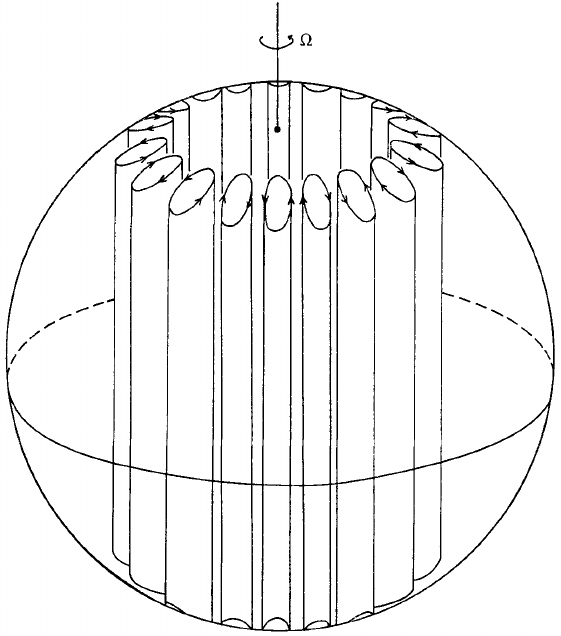
\includegraphics[width=1.05\textwidth]{sketches/busse_1975_onset.png}
 \caption{Sketch of the onset of convection for a rotating spherical shell. Convection columns form adjacent to the tangential cylinder \citep{busse1970thermal}. The columns can be visualized by different quantities. Here, they are sketched as contours of constant vorticity.}
 \label{fig:sketch_busse}
\end{minipage}
\hfill
\begin{minipage}[]{0.47\textwidth}
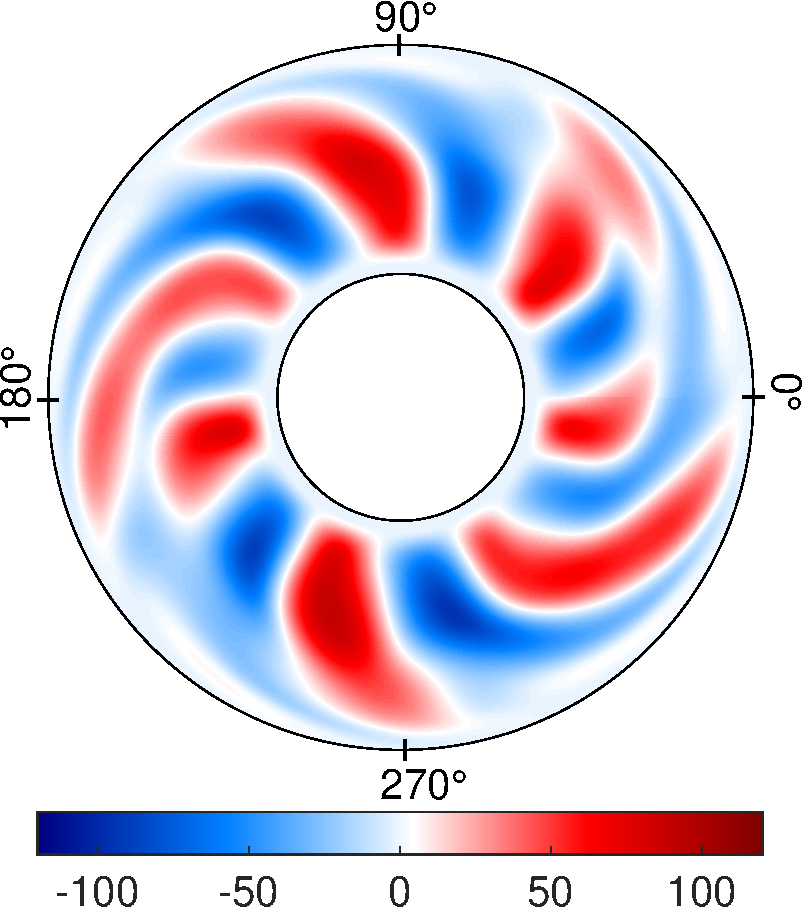
\includegraphics[width=\textwidth]{graphs/iso_440_ex_rad-crop.pdf}
\caption{Snapshot of the radial velocity in the equatorial plain (view from the north pole, like all other equatorial views in the following) for a uniform case with  $\textrm{Ra}_\textrm{\tiny T} = \textrm{Ra}_\textrm{total} = 4.4\cdot 10^6$, $\textrm{Pr}_\textrm{\tiny T} = 0.3$, $\textrm{Ek}=10^{-4}$ and $q^* = 0$. The convection columns are tilted and slightly deformed compared to Figure \ref{fig:sketch_busse}. }
\label{fig:radial_vel_ex}
\end{minipage}
\end{figure}
In a rotating system that is homogeneously forced, convection sets in in the form of a thermal Rossby wave \citep{busse1970thermal, busse2002convective}. The \textit{Taylor-Proudman theorem} (see section \ref{sec:thermal_wind}) imposes a column like structure to the system that is aligned with the axis of rotation ($z$-axis, see Figure \ref{fig:sketch_busse}) and drifts in azimuthal direction. \citet{busse2002convective} describes a mean flow instability that leads to differential rotation (the variation of azimuthal velocity with radius), evolving under the influence of a spherical geometry. Differential rotation presumably plays a central role in the magnetic field generation as it is an ingredient for the $\alpha$-effect \citep{roberts2007theory}. \\ \par

According to the analytical theories of \citet{jones2000onset} and \citet{dormy2004onset}, the azimuthal length scale of each convection column would be extremely small in case of the Earth's rotation rate. Therefore, this scenario is assumed to be unrealistic and the dominance of the relative influence of rotation compared to the one of buoyancy is questioned. The alternative is a rather three-dimensional, turbulent regime \citep{king2009boundary}, for which, on the other hand, the mechanism of the magnetic field production is an open question. \\ \par

\subsection{The geostrophic and the thermo-chemical wind balance}
\label{sec:thermal_wind}
The rotation rate of the LOC, measured in terms of the inverse of the non dimensional Ekman number $\textrm{Ek}^{-1}$, is very high (see section \ref{sec:parameters}). The \textit{Rossby number} $Ro = \frac{\mathcal{U}}{\Omega \mathcal{L}}$ quantifies the relative importance of the inertia force compared to the Coriolis force in the equation of momentum. If it is small, a system is predominantly rotationally constrained and this suggests simplifications, accordingly. The inertia term drops out and viscosity can be neglected as well due to $\textrm{Ek} = \frac{\nu}{\Omega D^2} \ll 1$. In the absence of gravitational instabilities, this yields the \textit{geostrophic balance}
\begin{equation}
\label{eq:geostrophy}
 -\frac{2}{\textrm{Ek}}\bm{e_z} \times \bm u= \bm \nabla \pi,
\end{equation}
where the rotational force is balanced by the pressure gradient \citep{vallis2006atmospheric, jones2007thermal}. The \textit{Taylor-Proudman theorem} follows from \eqref{eq:geostrophy}, if the curl is applied:
\begin{equation}
\label{eq:geostrophy2}
 (\bm{e_z} \cdot \bm \nabla) \bm u = 0.
\end{equation}
It states that variations in the velocity field parallel to the axis of rotation ($z$-axis) are suppressed. The system tends to take on two dimensional solution, although this is never realizable in a sphere which naturally has sloping boundaries \citep{busse2002convective}.\\
Relation \eqref{eq:geostrophy} slightly changes, if buoyancy forces due to temperature or compositional variations cannot be neglected. The \textit{thermo-chemical wind balance} then describes, how lateral gradients in $T$ and $C$ cause flow gradients parallel to the axis of rotation \citep{jones2007thermal}: 
\begin{align}
 \label{eq:thermal_wind}
-2 \frac{\partial \bm u}{\partial z}= (1-a) \textrm{Ek}\,\bm \nabla \times \left( \textrm{Ra}_\textrm{\tiny T}(\theta + t_2^2) + \textrm{Ra}_\textrm{\tiny C}\zeta \right)\bm r.
%=& \quad  (1-a) \textrm{Ek}\textrm{Ra}_\textrm{\tiny T}\left( \frac{1}{\textrm{} \vartheta}\frac{\partial (\theta + t_2^2)}{\partial \phi}\, \bm{e_\vartheta} + \frac{\partial (\theta + t_2^2)}{\partial \vartheta}\, \bm{e_\phi} \right)
\end{align}
It can be obtained, when adding the buoyancy term from equation \eqref{eq:force_balance4} to the force balance \eqref{eq:geostrophy} and taking the curl again. Equation \eqref{eq:thermal_wind} will be important in the following, because the conductive response to the heat flux pattern, $t_2^2$, prescribes lateral temperature gradients to the system. Additionally, dynamical variations $\theta$ and $\zeta$, especially along the polar coordinate $\vartheta$, are assumed to drive thermo-chemical winds in the sphere \citep{trumper2012numerical}. 

\subsection{The formation of radial flux patches by azimuthal temperature gradients in the equatorial plain}
\label{sec:radial_flow}
The non axisymmetric distribution of up- and downwellings in the time-averaged flow is a feature that is distinct to non homogeneous forcing provided by the heterogeneous core-mantle heat flux. \citet{zhang1992convection} and \citet{dietrich2016core} analytically show that the azimuthal position of in- and outward radial motion in the equatorial plain is determined by the azimuthal temperature gradient $\partial T / \partial \phi$. \\
Equation \eqref{eq:thermal_wind} is used as a starting point, whereupon only thermal forcing is regarded ($\textrm{Ra}_\textrm{\tiny C} = 0$). Since the $z$-axis plays a central role in the geostrophic context, cylindrical coordinates are used with $s$ as a radial distance from the axis of rotation. According to \citet{dietrich2016core}, the velocity field is split into a geostrophic part $\bm u^g$ and an ageostrophic part $\bm u^a$ with $\bm u = \bm u^g(s,\phi) + \bm u^a(s,z,\phi)$, where the geostrophic part per definition is independent of the $z$-position. To compute the geostrophic flow, the $z$-average of the $z$-component of \eqref{eq:thermal_wind} is needed,
\begin{equation}
\label{eq:wind_z1}
-2\,\Big \langle \frac{\partial u_z}{\partial z} \Big \rangle_z = {(1-a)\textrm{Ek}\textrm{Ra}_\textrm{\tiny T}} \, \langle \bm{e_z} \cdot \bm \nabla \times (\theta + t_2^2) \bm r \rangle_z,
\end{equation}
where the average of a function $f$ can be computed by
\begin{equation*}
 \langle f \rangle_z (s,\phi) = \frac{1}{2H} \int_{-H}^{+H} f(s,z,\phi) \, dz,
\end{equation*}
with $H = \sqrt{R_o^2 + s^2}$ as the half height of a cylinder at the radial position $s$ \citep{gillet2006quasi}. The right-hand-side (rhs) of \eqref{eq:wind_z1} can be transformed to (now in spherical coordinates)
\begin{equation}
\label{eq:wind_z2}
 \textrm{rhs} = {(1-a)\textrm{Ek}\textrm{Ra}_\textrm{\tiny T}} \, \bigg \langle \bm{e_z} \cdot \left( \frac{1}{\textrm{sin}\vartheta} \frac{\partial}{\partial \phi}(\theta + t^2_2)\, \bm{e_\vartheta} - \frac{\partial}{\partial \vartheta} (\theta + t^2_2) \, \bm{e_\phi} \right) \bigg \rangle_z
\end{equation}
The conductive temperature profile $t_2^2$ is symmetric with respect to the equator, hence its lateral gradient antisymmetric and it drops out when averaged over the $z$-axis. The temperature variation $\theta$ is likely to be distributed equatorial symmetric as well and therefore it is neglected, likewise. In cylindrical coordinates, \eqref{eq:wind_z2} now reads
\begin{equation}
\label{eq:wind_z3}
 \textrm{rhs} = (1-a) \textrm{Ek}\textrm{Ra}_\textrm{\tiny T} \frac{1}{s} \bigg \langle \frac{\partial}{\partial \phi} (\theta + t^2_2) \bm{e_z} \cdot \bm{e_\vartheta} \bigg \rangle_z.
\end{equation}
Following \citet{gillet2006quasi}, the left-hand-side of \eqref{eq:wind_z1} transforms to
\begin{equation}
\label{eq:wind_z4}
-2\,\Big \langle \frac{\partial u_z}{\partial z} \Big \rangle_z = -\frac{1}{H} \int_{-H}^{+H} \frac{\partial u_z}{\partial z} \, dz = -\left( - u_s^g \, \frac{2s}{H^2} \right).
\end{equation}
The slope of the spherical boundary is responsible for the fact, that a radial velocity component enters the $z$-averaged equation in order to balance the boundary condition.\\
In the equatorial plain, $\bm{e_z}\cdot \bm{e_\vartheta} = -1$, $r=s$ and the radial velocity $ u_s^g$ in cylindrical coordinates equals the radial velocity $u_r^g$ in spherical coordinates. It can now be expressed in terms of the azimuthal temperature gradient:
\begin{equation}
 \label{eq:ugr}
 u_r^g = -\frac{H^2}{2r^2}(1-a)\textrm{Ek}\textrm{Ra}_\textrm{\tiny T} \,\bigg \langle \frac{\partial}{\partial \phi}(\theta + t^2_2) \bigg \rangle_z.
\end{equation}
The position of the maximum (minimum) azimuthal temperature gradient should thus coincide with radial downwellings (upwellings) (see relation \eqref{eq:ugr} that contains a minus sign) in the equatorial plain. Since only the $z$-averaged / geostrophic  part of the velocity field $\bm u$ contains radial components (\citep{dietrich2016core}, $u_r^g$ is the full radial flow in this approximation. \\
\begin{figure}[t]
 \centering
 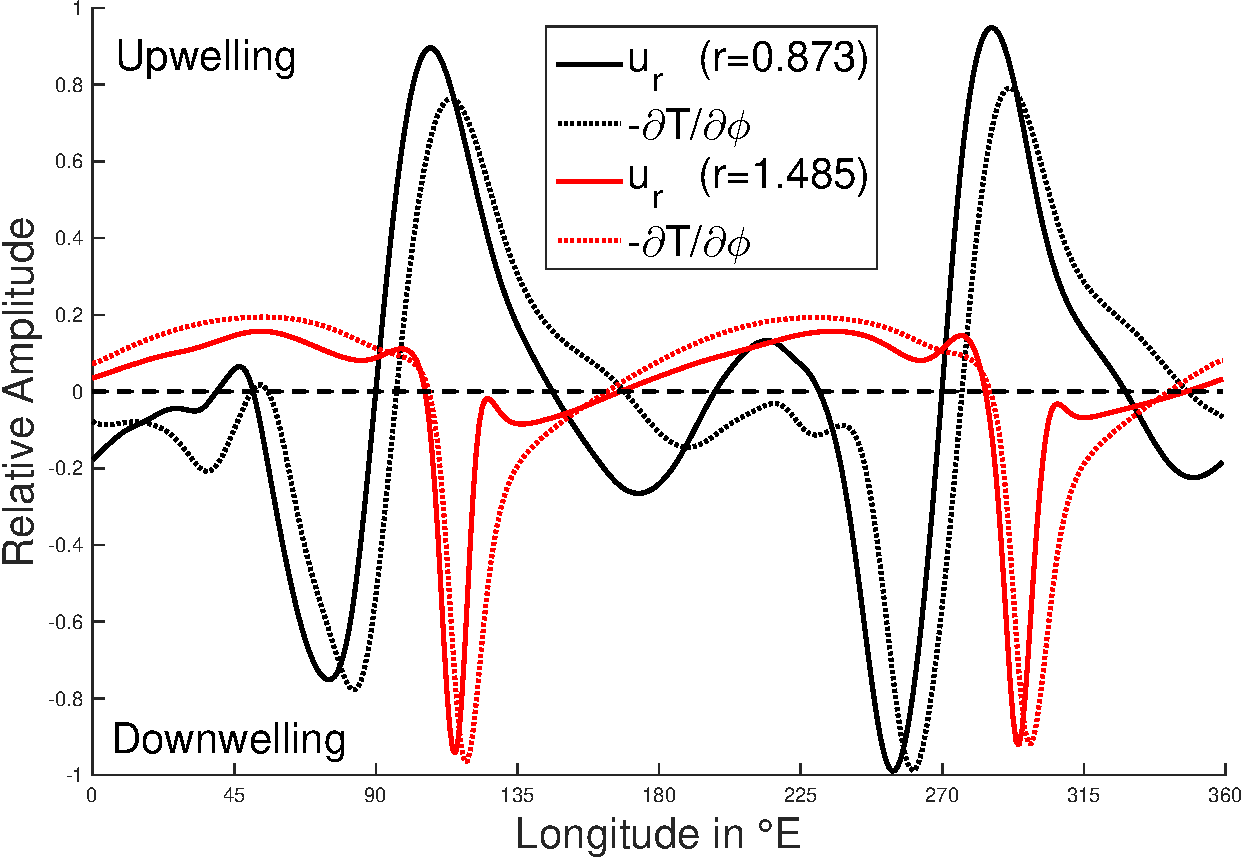
\includegraphics[width=\textwidth]{graphs/q2_200_ur_dTp-crop.pdf}
 \caption{Azimuthal profiles of the radial velocity $u_r$ (solid lines) and the negative azimuthal temperature gradient $-\partial (\theta + t_2^2)/\partial \phi$, here $-\partial T/\partial \phi$ (dotted lines), at mid depth (black, $r=0.873$) and at the top of the free stream near the CMB (red, $r=1.485$), normalized with respect to their individual maximum value. All values are measured in the equatorial plain. As parameters, $\textrm{Ra}_\textrm{\tiny T} = \textrm{Ra}_\textrm{total} = 2\cdot 10^6$ and $q^* = 2$ are used besides the Prandtl and Ekman number as mentioned above.}
\label{fig:ur_dTp}
 \end{figure}
Figure \ref{fig:ur_dTp} shows two azimuthal profiles of the the radial velocity $u_r$ (solid lines) and the negative azimuthal temperature gradient $\partial (\theta + t^2_2) / \partial \phi$ (dotted lines) in the equatorial plain. One is taken at mid depth (black lines), the other one on top of the free stream near the CMB (red lines). All values are normalized with respect to their maxima in order to make them comparable in one plot.\\ 
The forcing in this case is purely thermal with a Rayleigh number $\textrm{Ra}_\textrm{\tiny T} = \textrm{Ra}_\textrm{total} = 2\cdot 10^6$ that is slightly overcritical: $\textrm{Ra}_\textrm{\tiny T} \approx 3\cdot \textrm{Ra}_\textrm{crit}$. The critical Rayleigh number was taken from \citet{hori2012influence} who computed $\textrm{Ra}_\textrm{crit}$ for both, Neumann and and Derichlet type boundary conditions for the forcing component. \\ \par
\begin{figure}[t]
\centering
\begin{minipage}[left]{0.32\textwidth}
   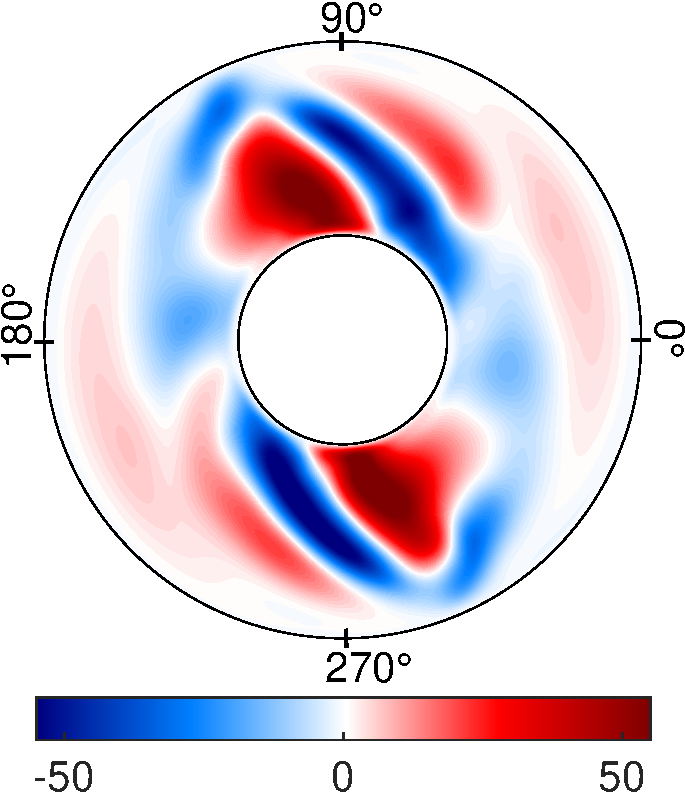
\includegraphics[width = \textwidth]{graphs/q2_200_d080_rad-crop.pdf}
   \caption*{(a) Radial Velocity}
\end{minipage}
\hfill
\begin{minipage}[center]{0.32\textwidth}
   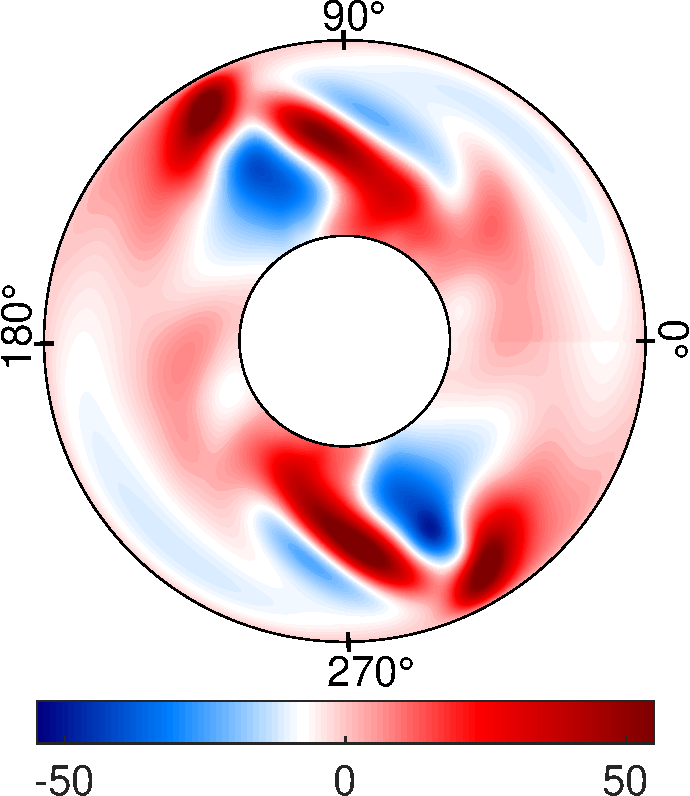
\includegraphics[width = \textwidth]{graphs/q2_200_dTp-crop.pdf}
   \caption*{(b) $\partial T / \partial \phi$, rescaled}
\end{minipage}
\hfill
\begin{minipage}[right]{0.32\textwidth}
    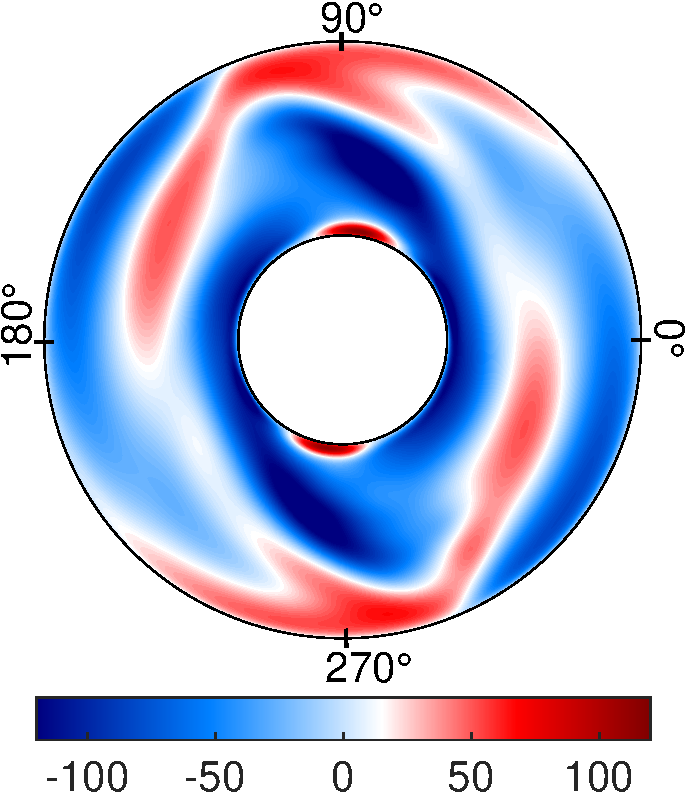
\includegraphics[width = \textwidth]{graphs/q2_200_d080_az-crop.pdf}
  \caption*{(c) Azimuthal velocity}
\end{minipage}
\caption{Equatorial contours of (a) the radial velocity, (b) the azimuthal temperature gradient $\partial (\theta + t_2^2) /\partial \phi$ and (c) the azimuthal velocity. The values in (b) are rescaled according to Equation \eqref{eq:ugr} (without the minus sign) in order to be comparable to (a). The case is the same as in Figure \ref{fig:ur_dTp}. }
\label{fig:equatorial_vel_temp}
\end{figure}
It becomes clear that the $\phi$-gradient of the temperature serves well as an explanation for the location of the two radial downwellings near the CMB. The two negative extrema of the radial velocity coincide nearly perfectly with the maxima of the azimuthal temperature gradient. Only the small kinks in front of and behind the extrema of $u_r$ cannot be explained by $\partial (\theta + t_2^2)/\partial \phi$ in this first order approach.\\ 
In a purely conductive regime with $\textrm{Ra}_\textrm{\tiny T} < \textrm{Ra}_\textrm{crit}$, the maxima of $\partial (\theta + t_2^2) / \partial \phi = \partial t_2^2 / \partial \phi$ (because $\theta=0$ in the subcritical case) would be located $45^\circ$ E of the heat flux maxima (located at $90^\circ$ E and $270^\circ$ E, see Figure \ref{fig:conductives} for the conductive temperature field) \citep{zhang1992convection}. The fact that the phase shift is only $30^\circ$ here (see Figure \ref{fig:ur_dTp}) can be attributed to the supercriticality of this case. More specifically, the azimuthal velocity field is responsible for the westward shift of the downwelling because it inhibits strong retrograde flow near the CMB around $135^\circ$ E (see Figure \ref{fig:equatorial_vel_temp}(c)). \\
In the upper region of the core, the two downwellings (around 120$^\circ$ and 300$^\circ$ E) are more pronounced than the complementary upwellings (around 45$^\circ$ and 225$^\circ$ E, see Figures \ref{fig:ur_dTp} and \ref{fig:equatorial_vel_temp}(a)). \citet{dietrich2016core} explain this asymmetry with the azimuthal part of the non linear temperature advection term $-\frac{\partial \theta}{\partial \phi}u_\phi$ (see Equation \eqref{eq:theta} that promotes positive azimuthal temperature gradients and therefore downwellings at the corresponding longitudes.  \\ \par

\begin{figure}[t]
 \centering
 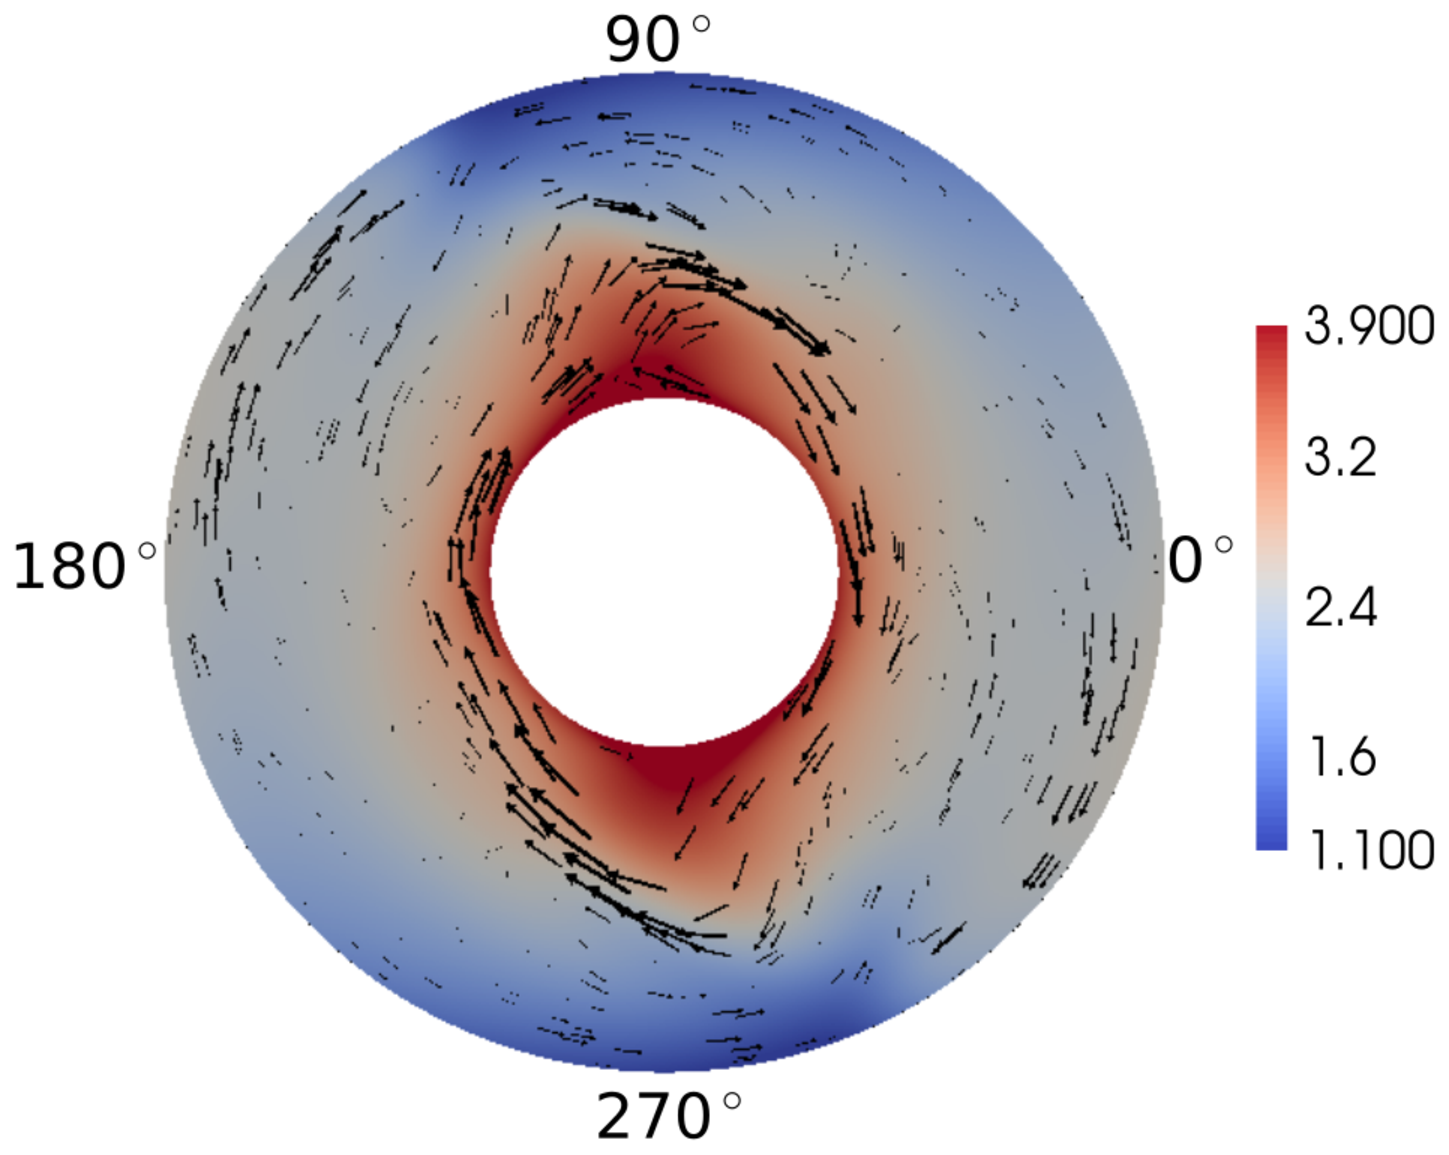
\includegraphics[scale=0.5]{graphs/q2_200_temp_vel-crop2.pdf}
 \caption{Horizontal velocity vectors in the equatorial plain, scaled by the corresponding flow magnitude. The background contour shows the full non dimensional temperature field $ T = \theta + T_\textrm{cond}$. The two strong upwelling plumes at the ICB (at $\sim 110^\circ$E and $\sim 290^\circ$E) and the bending jet like downwellings right above are clearly visible.}
\label{fig:flowfield_temp}
 \end{figure}

The radial flow in the deeper regions of the core (e.g. the solid black line Figure \ref{fig:ur_dTp}) has a more complex form and is thus not as directly as in the upper layers related to the $\mathcal{Y}_2^2$ heat flux pattern. Broad and pronounced upwellings develop right under the CMB downwellings at $\sim110^\circ$E and $\sim290^\circ$E. They are also visible in the temperature field in Figure \ref{fig:flowfield_temp} in form of hot plumes. \\
The downwellings observed at the CMB bend in jet like structures in retrograde direction towards the ICB (see Figure \ref{fig:equatorial_vel_temp}(a)). The bending happens due to strong zonal westward flows at mid depth at $\sim 90^\circ$E and $\sim 270^\circ$E, respectively (see Figure \ref{fig:equatorial_vel_temp}(c)).  \\ 
Although the flow structure in the deeper core regions is more complex than at the CMB, equation \eqref{eq:ugr} and therefore the thermo-chemical wind relation provide a good explanation for the radial flow field (compare Figure \ref{fig:equatorial_vel_temp}(a) and (b)). \\ \par

The small phase shift between $\partial T / \partial \phi$ and $u_r$, observable in Figure \ref{fig:ur_dTp} (dotted and solid lines), illustrates that the assumption of negligible viscosity (see section \ref{sec:thermal_wind}) is not fully justified in case of $\textrm{Ek} = 10^{-4}$. \citet{zhang1992convection} state that this shift vanishes if the rotation rate is further increased and therefore the influence of the viscosity decreased. \\ \par

The azimuthal flow in the equatorial plain is, in reaction to the radial flow, convergent (divergent) in the neighborhood of downwellings (upwellings). This can be observed either in the full horizontal flow field (Figure \ref{fig:flowfield_temp}) or in the radial and azimuthal flow fields (Figure \ref{fig:equatorial_vel_temp}(a) and (c)). The downwellings are each 'fed' from the lateral direction and vice versa.

\subsection{The effect of the flux pattern on the temperature field}
\label{sec:temp_field}
\begin{figure}[t]
 \begin{minipage}[left]{0.33\textwidth}
  \centering
  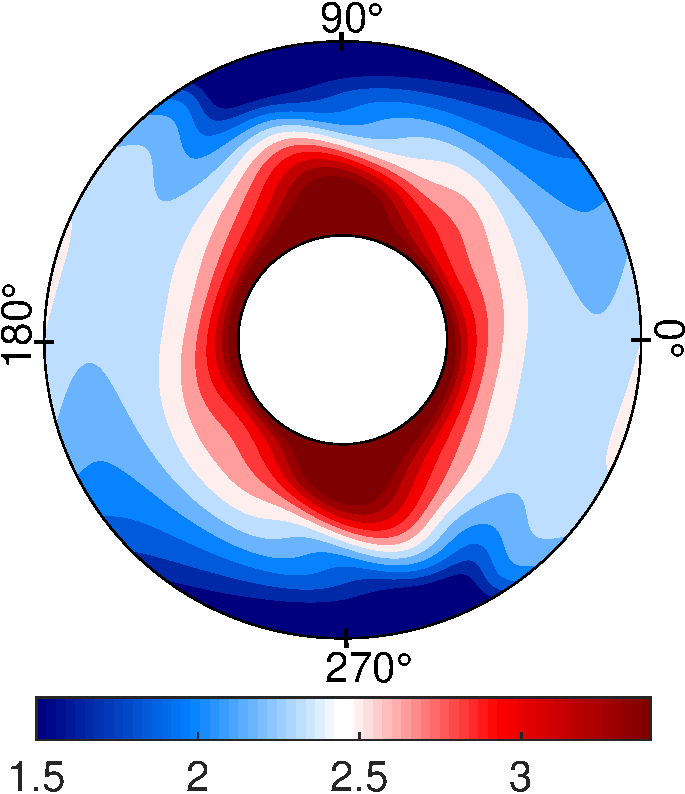
\includegraphics[width=\textwidth]{graphs/q2_200_eq_temp_field2-crop.pdf}
  \caption*{(a) Equatorial plain}
 \end{minipage}
 \hfill
\begin{minipage}[right]{0.63\textwidth}
 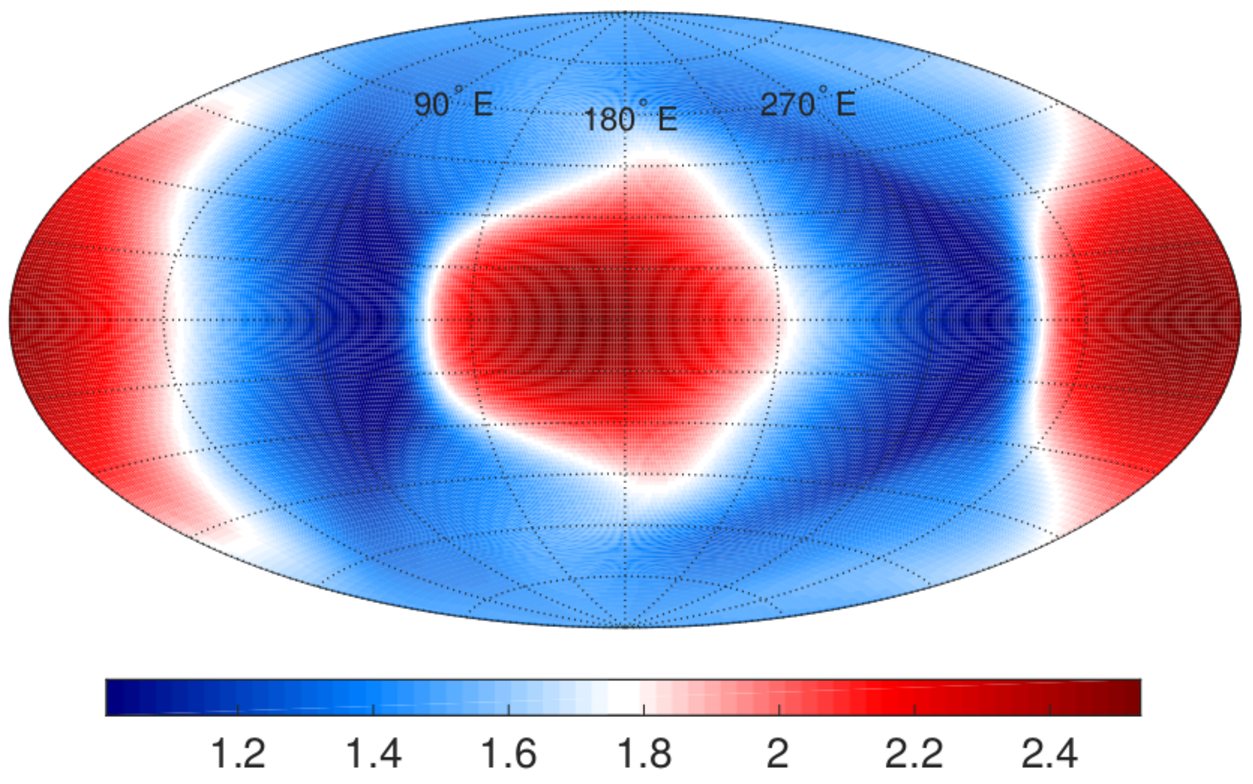
\includegraphics[width=\textwidth]{graphs/q2_200_tammer-crop.pdf}
 \caption*{(b) Surface projection at the CMB}
\end{minipage}
\caption{Full temperature field $ T = \theta + T_\textrm{cond}$ for the same case as above in (a) the equatorial plain and (b) as a surface projection right under the CMB. (a) is the same graph as in Figure \ref{fig:flowfield_temp}, but the color map is 'shortened' in order to pronounce the the phase shift of the temperature field. }
\label{fig:q2_200_temp}
\end{figure}
Figure \ref{fig:q2_200_temp}(a) shows the same equatorial view on the temperature field as Figure \ref{fig:flowfield_temp} in the previous section. The color map was slightly rescaled to make the phase shift between the temperature maxima at the CMB at $\sim 170^\circ$ and $\sim 350^\circ$ and the heat flux maxima (at $\sim 90^\circ$ and $\sim 270^\circ$) visible. The reason for the phase shift lies in the flow field and can be found in the previous chapter: Strong radial motion occurs predominantly in the region under the heat flux maxima. The up- and downwellings visible in Figure \ref{fig:flowfield_temp} intensify the cooling mechanism, thus go along with a colder core region. The hot regions coincide with strong azimuthal motion along the CMB that inhibit the transport of heat out of the core. (EKMAN dependence ???) \\
The surface projection of the temperature field at the CMB (Figure \ref{fig:q2_200_temp}(b)) confirms that the temperature field in the slightly super critical case nearly is a phase shifted version of the conductive temperature field (Figure \ref{fig:conductives}(b)) \citep{zhang1992convection}. 

\subsection{Columns of constant vorticity}
\label{sec:vortex_clolumns}
As mentioned above, convection in rapidly rotating systems is organized in a column like structure at onset \citep{busse1970thermal}. The question whether this structure is maintained, even in the highly super critical LOC, has important implications for the understanding of the geodynamo. The so called \textit{vortex columns}, visualized in Figures \ref{fig:sketch_busse} and \ref{fig:vort_uniform} in the equatorial plain, play a key role in the magnetic field production. \\
Although motion parallel to the $z$-axis is strongly constrained by rotation (see Equation \eqref{eq:geostrophy2}), the spherical form of the boundaries necessarily relaxes this constraint locally and vertical flow is unavoidable \citep{busse2002convective, gillet2006quasi}. An important example for the relaxation of the Taylor-Proudman theorem in this context is the \textit{secondary circulation} inside of vortex columns \citep{olson1999numerical, aubert2008magnetic, christensen2011geodynamo}, sketched in Figure \ref{fig:secondary_circulation}.\\
\begin{figure}[H]
 \begin{minipage}[left]{0.49\textwidth}
  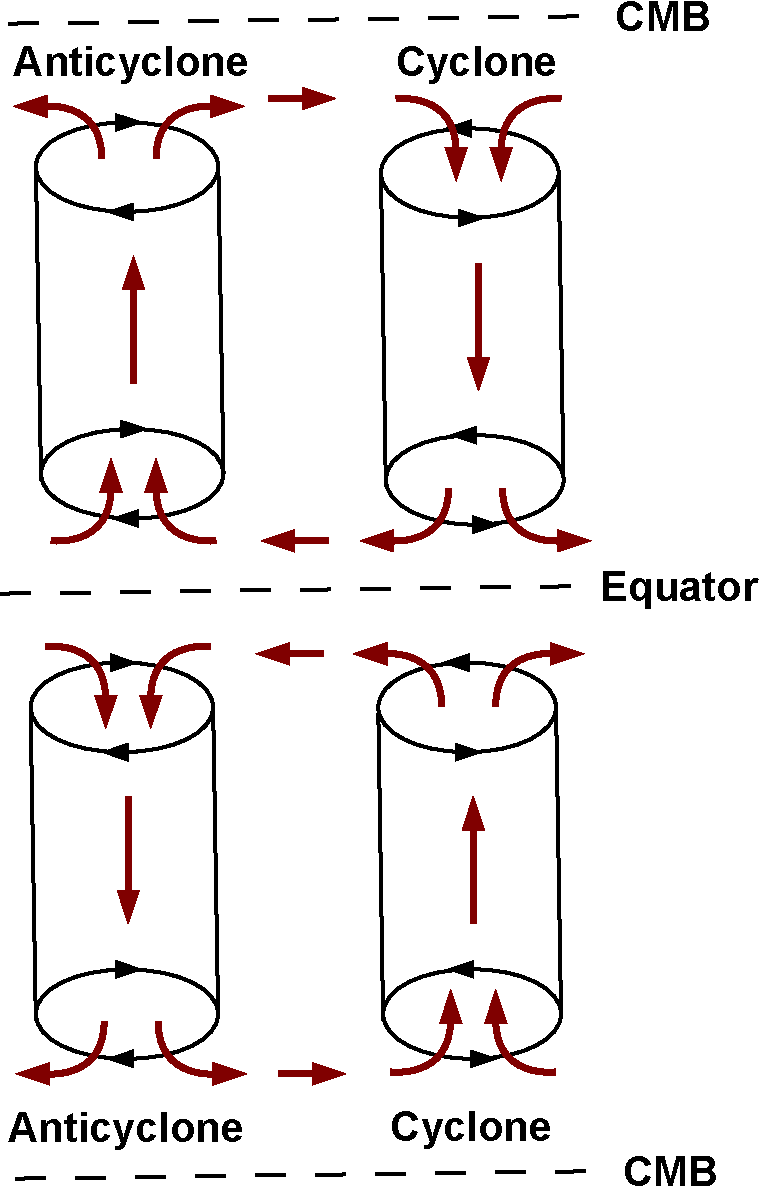
\includegraphics[width =  \textwidth]{sketches/secondary_circulation-crop.pdf}
  \caption{Sketch of the secondary circulation induced by a pair of a cyclonic and an anticyclonic vortex. The two convection columns can be imagined as part of the sketch in Figure \ref{fig:sketch_busse}, a situation typical for the onset of convection.}
  \label{fig:secondary_circulation}
 \end{minipage}
\hfill
\begin{minipage}[right]{0.48\textwidth}
\textit{Ekman pumping} and \textit{suction} are boundary layer effects that are distinct to systems with no-slip conditions (as in this study, see section \ref{sec:bc}). They evolve in the interplay between the rotation dominated bulk and the viscosity dominated Ekman layer. In \textit{cyclones}, i.e. vortex columns with positive vorticity $\omega > 0$, Ekman pumping induces a vertical flux away from the CMB towards the equator. Ekman suction causes motion towards the CMB in \textit{anticyclones}, where $\omega < 0$. Although both mechanisms take place in the boundary layers, they potentially induce vertical motion in the whole column. A more detailed description can be found in \citet{pedlosky2013geophysical}.\\
The variation of buoyancy along the $z$-axis inside of a vortex column acts as a second source of vertical motion \citep{olson1999numerical}. As in the case of Ekman suction and pumping, this motion is oriented equatorwards in cyclones and away from the equator in anticyclones. It is independent of the viscous boundary condition and therefore it makes this discussion applicable to a wider range of model configurations. 
\end{minipage}
\end{figure}
Figure \ref{fig:secondary_circulation} shows how a cyclone causes a divergent flow at the equator, whereas an anticyclone acts converging at the equator. The opposite is true near the CMB. A cyclone and an anticyclone together form a \textit{circular} motion that superimposes the primary vortial motion. The interaction of a vorticity carrying fluid column and a vertical flow produces helicity $\mathcal{H}$. Besides the differential rotation that is necessary for the $\omega$-effect, the presence of helicity is a condition for the occurrence of the (macroscopic) $\alpha$-effect \citep{roberts2007theory, christensen2011geodynamo, jones2011planetary}. For a detailed explanation of the two effects and their importance for the geodynamo, the reader is referred to the literature cited above. For the moment it is sufficient to know that the $\omega$-effect is a potential source for toroidal magnetic field, whereas the $\alpha$-effect theoretically is responsible for both, the production of toroidal and poloidal field. \\ \par

\subsection{Stationary vortex columns attached to mantle heterogeneities}
\label{sec:attached_columns}
\begin{figure}[t]
\begin{minipage}[left]{0.47\textwidth}
 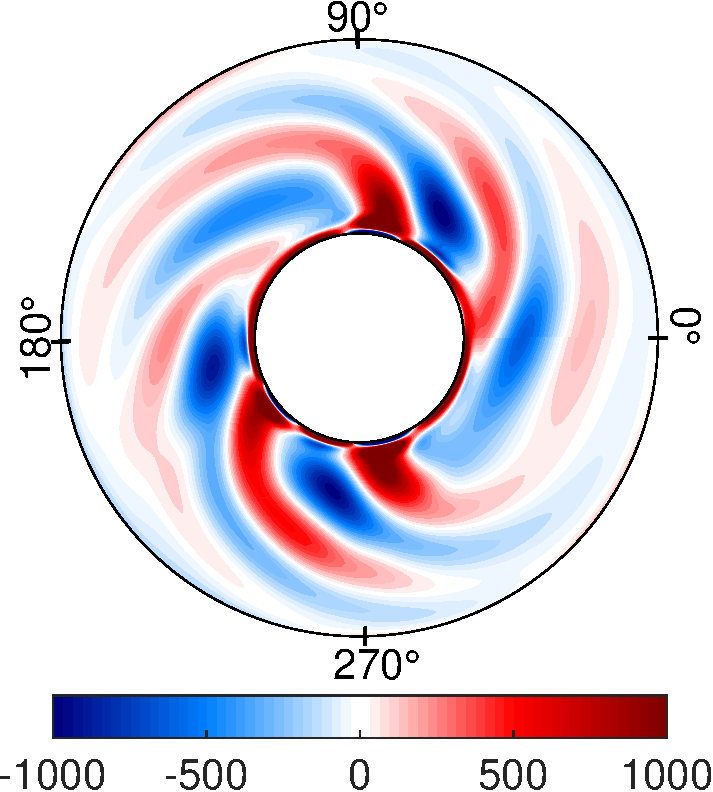
\includegraphics[width =\textwidth]{graphs/vorticity/q0_100_ex_vort-crop.pdf}
 \caption{Snapshot of the $z$-component of vorticity in the equatorial plain for a slightly super critical, uniform case: $\textrm{Ra}_\textrm{\tiny T} = 10^{6}$.  }
 \label{fig:vort_uniform}
\end{minipage}
\hfill
\begin{minipage}[right]{0.47\textwidth}
 \includegraphics[width=0.96\textwidth]{graphs/vorticity/q2_200_d080_vort-crop.pdf}
 \caption{Long-term averaged equatorial contour of the $z$-vorticity for the same case as described in Figure \ref{fig:equatorial_vel_temp}. The vorticity in the boundary layers is not resolved.}
 \label{fig:q2_200_d080_vort}
\end{minipage}
\end{figure}
The well structured Rossby wave solution is perturbed, if heterogeneous heat flux conditions are applied at the CMB. Nevertheless, columns of constant vorticity play an important role in the solution. The long-term averaged data bears a non axisymmetric vorticity pattern that can be related to the geometry of the CMB heat flux. This pattern contains \textit{stationary vortex columns} elongated through the whole sphere parallel to the axis of rotation. In contrast to that, all uniform cases regarded (e.g. the snapshot in Figure \ref{fig:vort_uniform}) yield axisymmetric distributions of vorticity in long-term averages because the Rossby wave solution constantly moves in azimuthal direction \citet{busse2002convective}. \\
The secondary circulation is expected to have an effect on the flow that can be localized at a fixed position in the spherical shell, it is \textit{locked} to the mantle \citep{gibbons2000convection}. 

\begin{figure}[t]
 \centering
 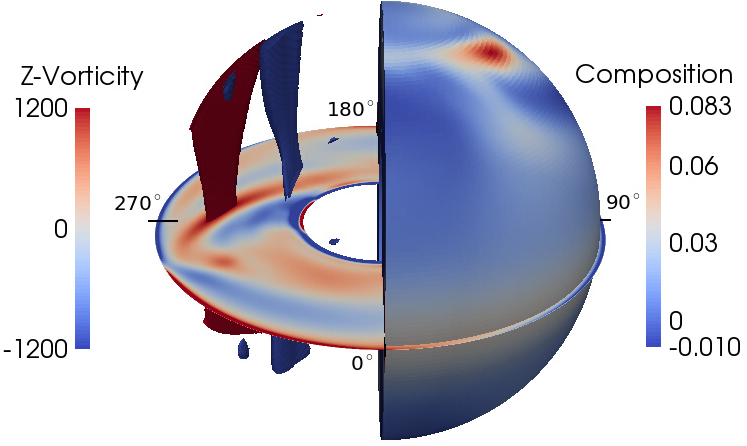
\includegraphics[scale = 0.7]{graphs/vorticity/q2_200_vort.png}
 \caption{\textbf{Left hemisphere}: $z$-component of the vorticity in the equatorial plain (see Figure \ref{fig:q2_200_d080_vort}) and contour surfaces at $\omega_z = -1200$ (blue) and $\omega_z = 1200$ (red). \textbf{Right hemisphere}: Compositional perturbation $\zeta$ close to the CMB at $ r = 1.5$. As parameters, $\textrm{Ra}_\textrm{total}=  2\cdot 10^6$, $\delta = 0.95$ and $q^* = 2$ are chosen.}
 \label{fig:vort_chem}
\end{figure}
The interplay of the azimuthal and the radial velocity field in the equatorial plain (Figure \ref{fig:equatorial_vel_temp}(a) and (b)) causes the vorticity distribution that is shown in Figure \ref{fig:q2_200_d080_vort}. Tilted patches of strong negative vorticity close to the ICB lie beneath prograde jets of positive vorticity right under the heat flux maxima at $90^\circ$E and $270^\circ$E. Additionally, a band of negative vorticity is located between $90^\circ$ and $180^\circ$E and $270^\circ$ and $360^\circ$E. \\
In Figure \ref{fig:vort_chem}, the long-term averaged vorticity distribution of a thermo-chemically driven case is shown in the left hemisphere, whereas the right hemisphere depicts the compositional perturbation $\zeta$. The forcing is predominantly of thermal origin, only a portion of 5\% uniform compositional forcing was included. The total Rayleigh number remains $\sim 3$ times supercritical in order to be comparable to the previous case. The vorticity contours in the left hemisphere yield the stationary vortex columns attached to the heat flux maxima mentioned above. An anticyclone (blue) elongates close to the tangential cylinder from the northern to the southern CMB. A cyclonic column (red) lies parallel to the anticyclone in the radially outward direction. The right hemisphere underlies the same vorticity distribution (see the symmetry in Figure \ref{fig:q2_200_d080_vort}). Here, the compositional perturbation yields a maximum at the intersection of the blue anticyclone with the CMB and a deficit when going towards the equator, i.e., where the red cyclone intersects the CMB. \\
The excess and deficit composition results from the divergent and convergent flow at the peak of the anticyclone and the cyclone, respectively. The corresponding mechanism is sketched in Figure \ref{fig:secondary_circulation}. In this case, the compositional forcing rather acts as 'tracer' that visualizes the vertical transport from the ICB, where the chemical component is released, to the CMB. A portion of 5 \% compositional forcing is expected to have only a little effect on the dynamics of the system compared to the purely thermal case from above.

\section{Thermo-chemical dynamo action}

\subsection{The influence of chemical forcing on magnetic field properties}

\section{Summary}

\section{Conclusion and Outlook}


\newpage
 \bibliography{literatur}
 \bibliographystyle{apalike}


%\end{thebibliography}
\end{document}